% !TEX encoding = UTF-8 Unicode

%%%%%%%%%%%%%%%%%%%% author.tex %%%%%%%%%%%%%%%%%%%%%%%%%%%%%%%%%%%
%
% sample root file for your "contribution" to a proceedings volume
%
% Use this file as a template for your own input.
%
%%%%%%%%%%%%%%%% Springer %%%%%%%%%%%%%%%%%%%%%%%%%%%%%%%%%%


\documentclass[conference]{IEEEtran}
%
% RECOMMENDED %%%%%%%%%%%%%%%%%%%%%%%%%%%%%%%%%%%%%%%%%%%%%%%%%%%
%

% to typeset URLs, URIs, and DOIs
% https://www.overleaf.com/learn/latex/Hyperlinks
\usepackage{hyperref}
\hypersetup{
    colorlinks=true,
    linkcolor=blue,
    filecolor=magenta,      
    urlcolor=cyan,
    pdftitle={Overleaf Example},
    pdfpagemode=FullScreen,
    }

\def\UrlFont{\rmfamily}

\usepackage[T1]{fontenc}
\usepackage[utf8]{inputenc}
\usepackage[textsize=scriptsize]{todonotes}
\usepackage{gensymb}
\usepackage{array,multirow}
\usepackage{caption} 
\captionsetup[table]{skip=10pt}
\usepackage{makecell}

\usepackage{cite}
\usepackage{amsmath,amssymb,amsfonts}
\usepackage{bm}
\usepackage{algorithmic}
\usepackage{graphicx}
\usepackage{textcomp}
\usepackage{xcolor}
\def\BibTeX{{\rm B\kern-.05em{\sc i\kern-.025em b}\kern-.08em
    T\kern-.1667em\lower.7ex\hbox{E}\kern-.125emX}}

\usepackage{graphicx}
\graphicspath{ {./img/} }

\renewcommand{\labelenumii}{\theenumii}
\renewcommand{\theenumii}{\theenumi.\arabic{enumii}.}

\begin{document}
%
\title{Duckietown project pros and cons}

\author{

\IEEEauthorblockN{1\textsuperscript{st} Marek Długosz}
\IEEEauthorblockA{\textit{AGH University of Science and Technology}\\
Cracow, Poland \\
mdlugosz@agh.edu.pl \\
0000-0001-6827-9149}

\and

\IEEEauthorblockN{2\textsuperscript{nd} Paweł Skruch}
\IEEEauthorblockA{\textit{IEEE Senior Member}}
\IEEEauthorblockA{\textit{AGH University of Science and Technology} \\
Cracow, Poland \\
pawel.skruch@agh.edu.pl\\
0000-0002-8290-8375}

\and

\IEEEauthorblockN{3\textsuperscript{rd} Marcin Szelest}
\IEEEauthorblockA{\textit{IEEE Senior Member}}
\IEEEauthorblockA{\textit{AGH University of Science and Technology} \\
Cracow, Poland \\
pawel.skruch@agh.edu.pl\\
0000-0002-0522-1270}

\and 

\IEEEauthorblockN{4\textsuperscript{th} Artur Morys-Magiera}
\IEEEauthorblockA{\textit{AGH University of Science and Technology} \\
Cracow, Poland \\
amorys@student.agh.edu.pl\\
0000-0002-2137-8841}

}

\maketitle              % typeset the title of the contribution

\begin{abstract}
The Duckietown project is a project aimed at developing a software and hardware platform for robot autonomy education and research. The project includes the design of robots, a mockup of cities, and additional infrastructure elements such as those for Watchtower navigation. The platform also includes a software-based Duckebot-GYM robot simulator that allows simulation of robot operation in a virtualized environment. It also includes the use of a Jetson Nano platform to control the duckiebot robot with hardware GPU support.
\end{abstract}


% We would like to encourage you to list your keywords within
% the abstract section using the \keywords{...} command.
\begin{IEEEkeywords}
autonomous, autonomous vehicle, electrical vehicle, control system
\end{IEEEkeywords}
%
\section{Introduction}
The basic skill of engineers is to solve practical problems. The study of engineering should provide opportunities for students to acquire these skills through the implementation of a variety of practical activities. Depending on the field of engineering, practical activities for students may be easier or more difficult to implement. A field of engineering science that requires expensive equipment and highly qualified personnel is the field of autonomous vehicles and robots. 
In such cases, laboratory workstations that use models of robots or autonomous vehicles along with a model of the environment in which they operate are of great help.
One such project that realizes the above is the \emph{Duckietown} project\footnote{https://duckietown.org} \cite{tani2017duckietown}.

The Duckietown project was created in 2016 at the University of Massachusetts Institute of Technology (MIT) as part of a class for students \cite{paull2017duckietown}. The goal of the project was to develop a software and hardware platform for the education and research on robot autonomy. Currently, the project is being developed at ETH. The project includes the design of Duckiebot robots, a mock-up of Duckietown cities, and additional infrastructure elements, such as for Watchtower navigation. The project also includes a software-based Duckiebot-GYM robot simulator that allows simulation of robot operation in a virtualized environment. 
In 2017, project leaders Liam Paull (Montréal), Andrea Censi and Jacopo Tani (ETH), and Matthew Walter (TTIC) decided for the first time to use the Duckietown platform in classes with students at four different universities ETH Zürich, Université de Montréal, TTI Chicago and NCTU. As a result, students from these universities had the opportunity to compare solutions to various problems in the field of autonomous robots among themselves. 2018 has seen a rapid increase in interest in the Duckietown project from universities and companies. The Duckietown platform needed to become more affordable, easier to acquire, and better quality so that it could support teaching and research in a more general way. As a result, a campaign was launched on the Kickstarer platform to raise funds to further develop the project. The following year, 2019 saw the debut of the AI Driving Olympics (AI-DO) competition at the Neural Information Processing Systems Conference (NeurIPS) in Montreal \cite{censi2019ai}. It is worth noting that this was the first competition held at a machine learning conference with real robots. The following years saw further development of the project, the development of a new version of the Duckiebot robots, the presentation of the platform at the Science Museum of London exhibition, and the development of an online course on the \emph{edX} platform called \emph{"Self-Driving Cars with Duckietown"}\footnote{https://www.edx.org/search?q=Self-Driving+Cars+with+Duckietown} which is very popular.

The second version of the Duckiebot robots is now available, which uses the JetsonNano computer for control. The JetsonNano platform enables the use of neural networks with hardware GPU support to control the Duckiebot robot. 

The article is organized as follows: section \ref{sec:hardware} describes the hardware part of the project including Duckiebot robots, Duckietown infrastructure elements, and Watchtower with the noted drawbacks of the project. Section \ref{sec:software} describes the software part of the project, indicating the advantages and disadvantages of the solutions adopted.
Section \ref{sec:documentation} describes the available documentation of the project and finally section \ref{sec:conclusion} summarizes the strengths and weaknesses of the project.

\section{Hardware platform}\label{sec:hardware}
The design of the body, the selection of robot components such as sensors, drives, and power supply are crucial in the later life of robots. Even the best theoretical design of a robot may not work satisfactorily if inadequate components are used to implement it. 
The Duckiebot robot is purchased as a self-assembly kit. The kit includes all the necessary components needed to assemble the Duckiebot robot. The assembly does not pose any problems, and the very well-prepared assembly documentation should be emphasized here. The DB21M version of the Duckiebot robot is equipped with a differential drive, one RGB camera, LED-RGB LEDs, two motors, a distance sensor, a set of motors with gears and encoders, two drive wheels and support ball (freewheel), an NVIDIA Jetson Nano computer, one button, and an OLED display. The assembled Duckiebot robot is shown in Figure \ref{fig:robot-duckiebot}.

\begin{figure}
    \centering
    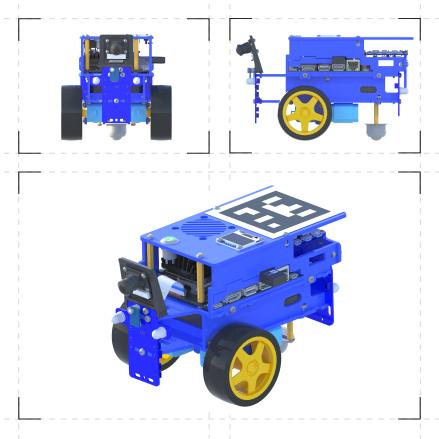
\includegraphics[width=1.0\columnwidth]{d3.jpg}
    \caption{Robot Duckiebot DB21M.}
    \label{fig:robot-duckiebot}
\end{figure}

\subsection{Body}
The body of the Duckiebot robot is made entirely of plastic parts. This choice of material certainly reduces the price of the robot, but also affects its mechanical strength. Figure \ref{fig:chassis-problem} shows typical problems of the Duckiebot robot body.

\begin{figure}
    \centering
    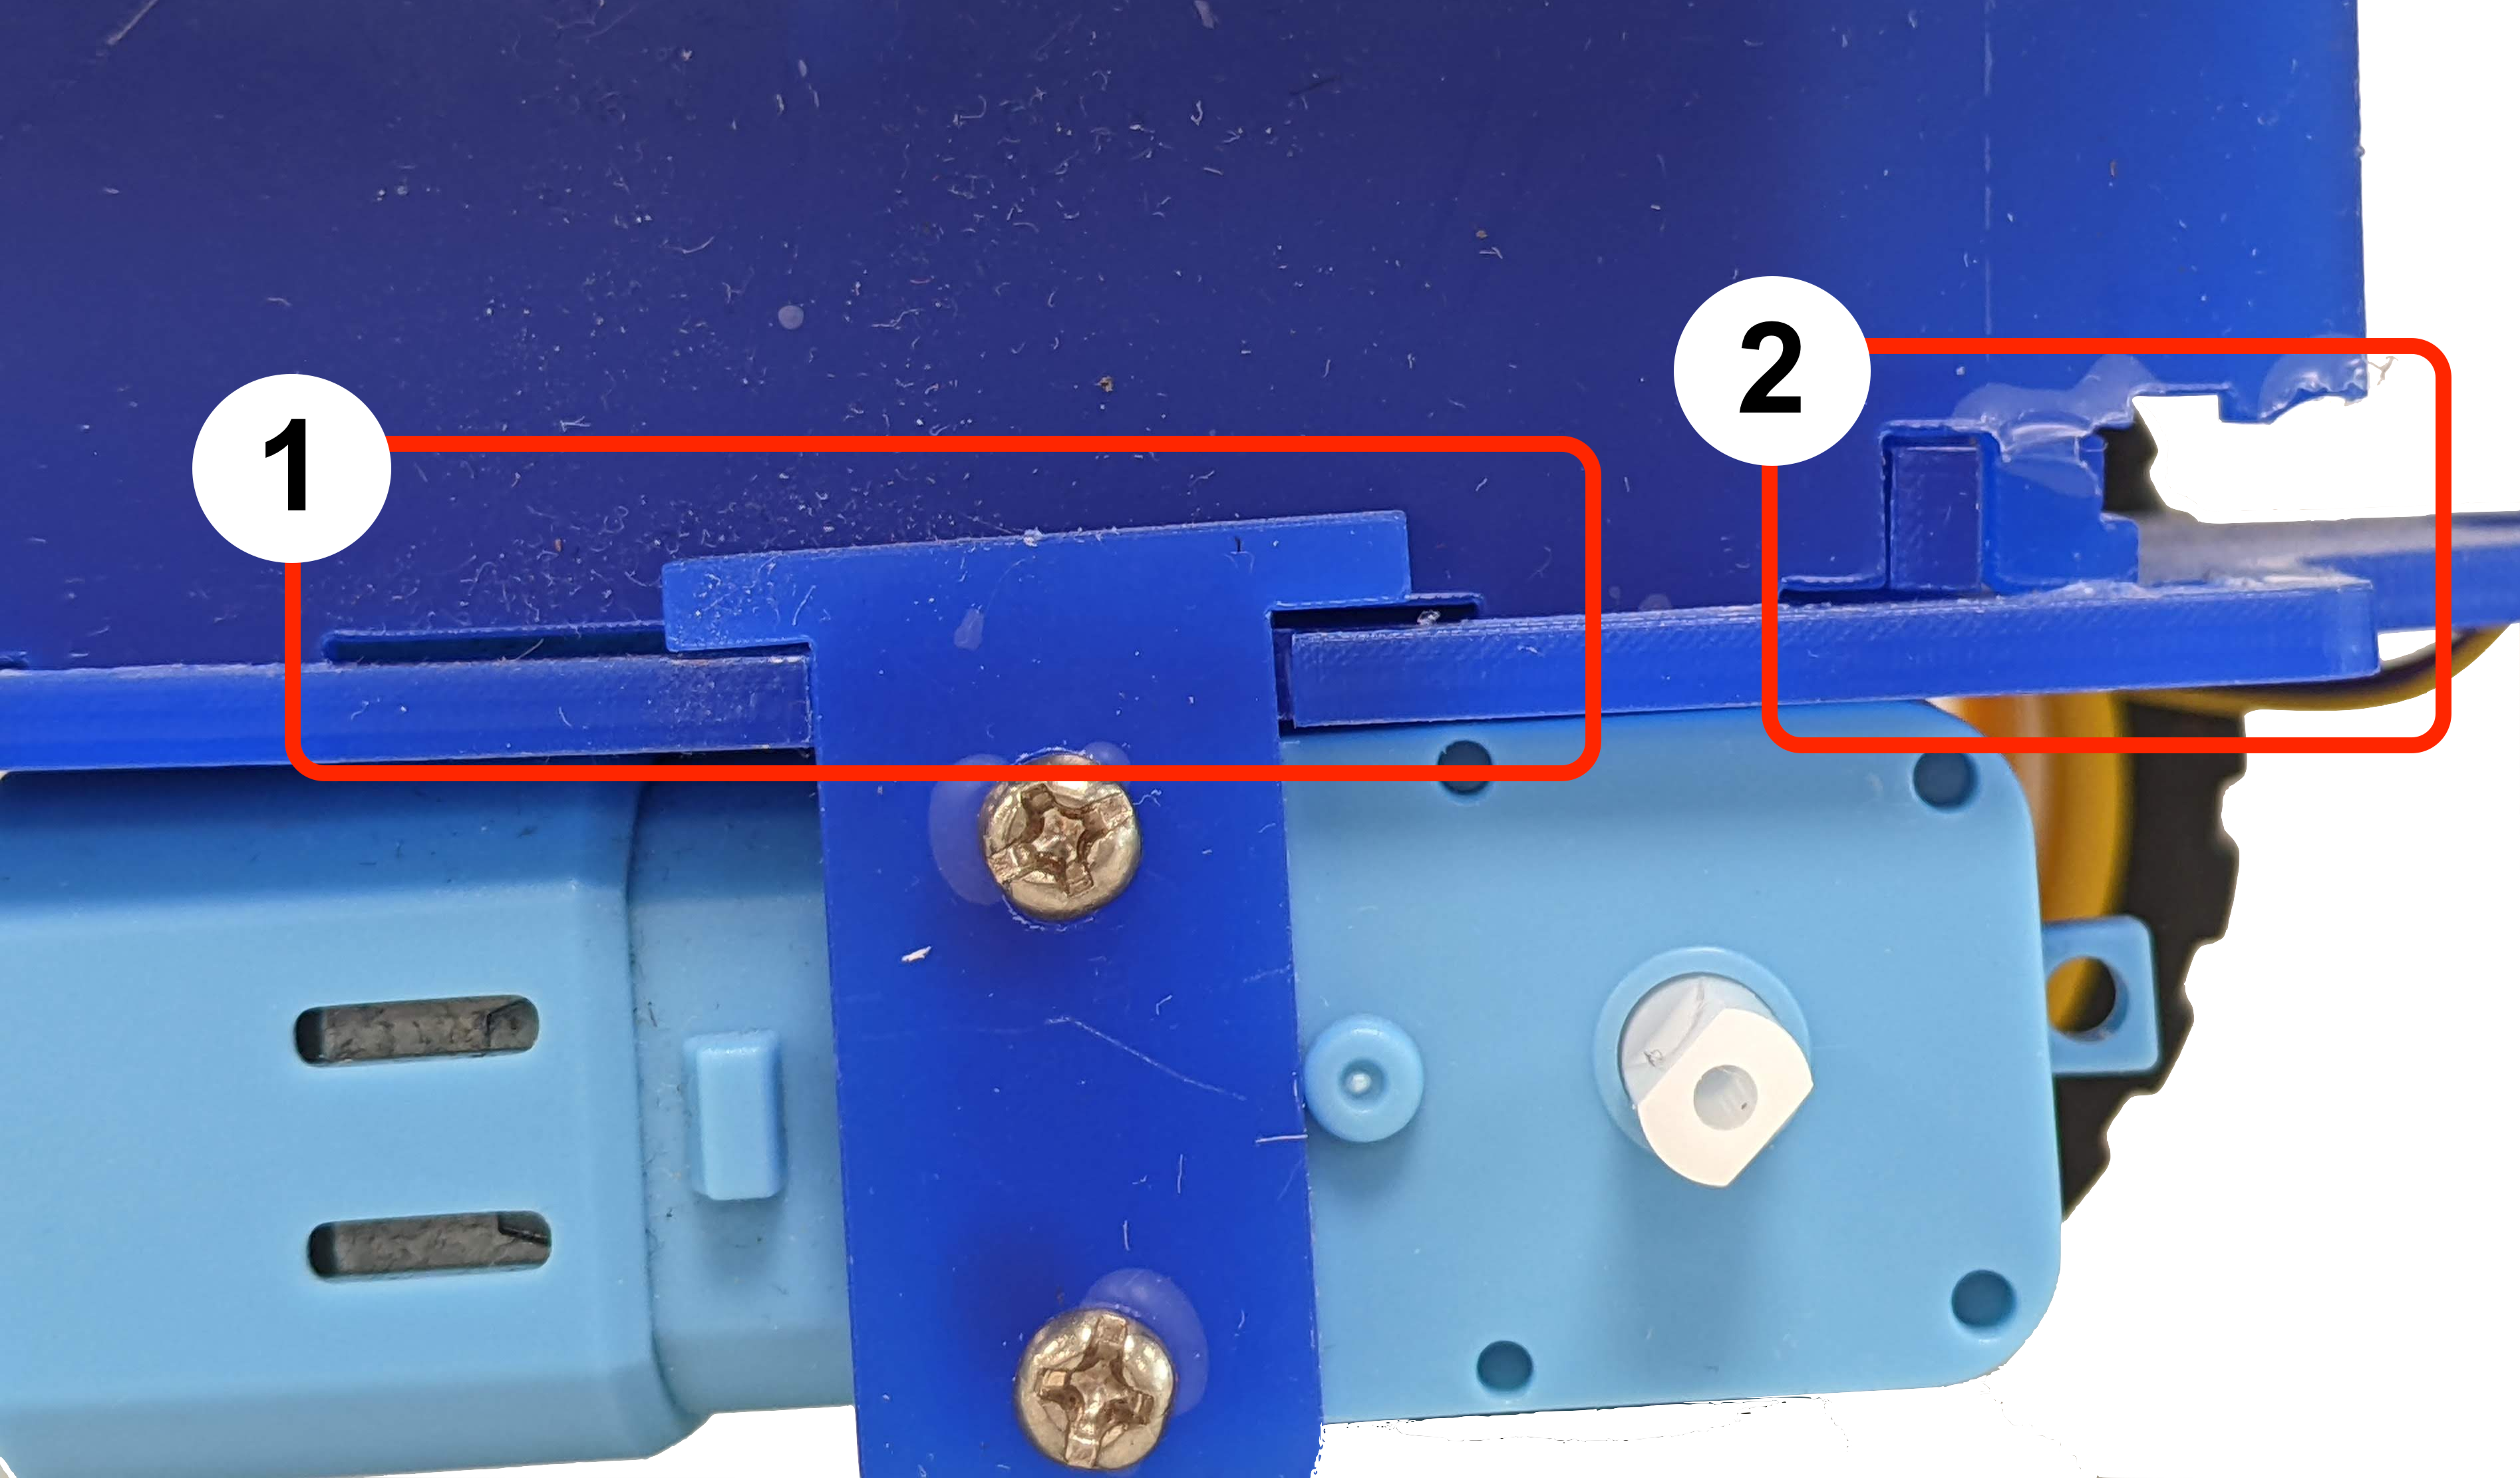
\includegraphics[width=1.0\columnwidth]{chassis1.png}
    \caption{Fragment of the plastic body of the robot Duckiebot.}
    \label{fig:chassis-problem}
\end{figure}

The first of the problems noted is the poor quality of the fit of the various parts of the Duckiebot robot body. It is due to the insufficient size of the space in which the battery is located. The design and execution of the body did not foresee that the nuts that are located in this space also have their own height, which makes the battery take up a little more space than is apparent from its external dimensions. This results in gaps (detail No. 1 in Fig. \ref{fig:chassis-problem}) and a less rigid attachment of the motor to the body. Due to the mechanical properties of the material from which the body is made (plastic), and the location of the nut holes too close to the edges of the body components, they tend to break out (detail No. 2 in Fig. \ref{fig:chassis-problem}). The use of plastic screws (not all of them) to connect body parts is also a certain shortcoming.

Another problem with the body is the lack of adequate lateral stiffness (along the Y axis), which results in the fact that the drive wheels are deformed outward (\emph{negative camber}), see fig. \ref{fig:negative-camber}. 

\begin{figure}
    \centering
    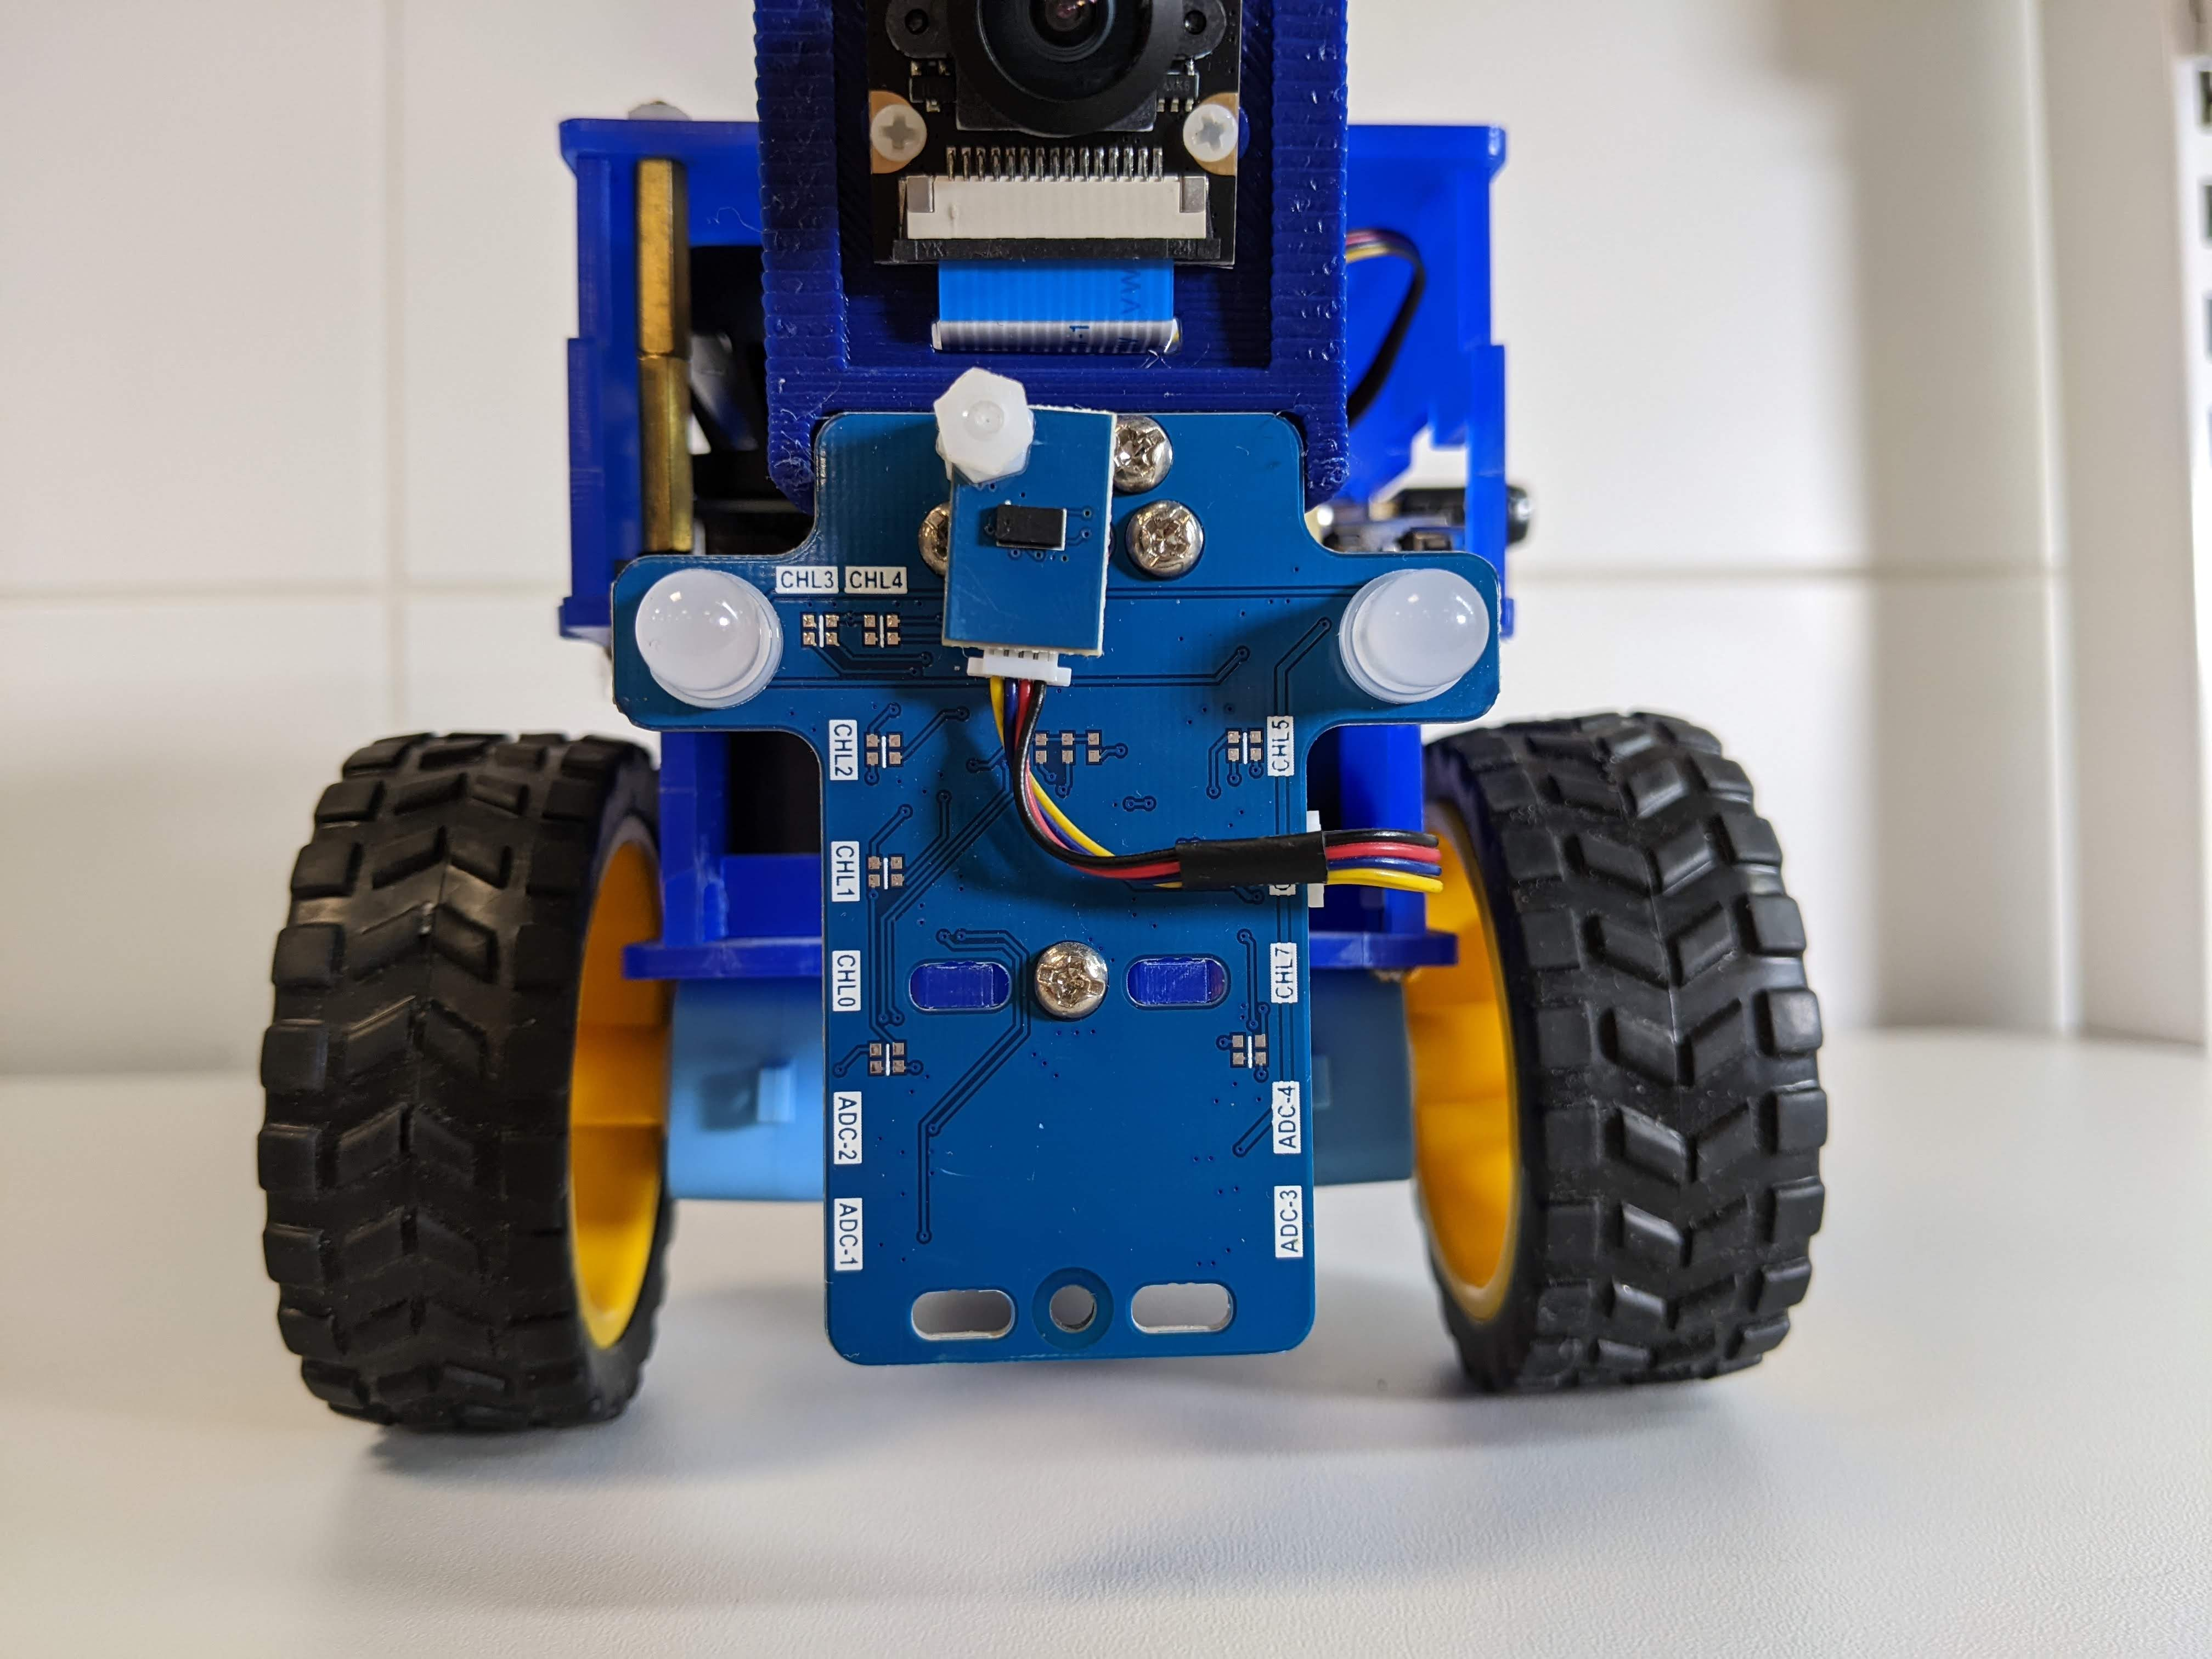
\includegraphics[width=1.0\columnwidth]{PXL_20221207_092836283.png}
    \caption{Negative camber of the of Duckiebot robot wheels.}
    \label{fig:negative-camber}
\end{figure}

The negative camber of the wheels makes the Duckiebot robot oversteer, which at first may seem like an advantage. However, considering the surface on which the Duckiebot robot moves (see section \ref{subsec:plane}) and the asymmetry in the operation of the motors (at the same supply voltage, the speeds of the motors are not identical), oversteering is a disadvantage rather than an advantage. It causes even a minimal disturbance (from uneven pavement and asymmetrical operation of the motors) to result in the Duckiebot robot abruptly changing its direction of movement so that the control system is unable to steer the robot correctly. 

The traction properties of Duckiebot robots can be improved by connecting the motor mounts with a crossbar that stiffens the motor mounts to prevent negative camber of the wheels; see fig. \ref{fig:stiffening-crossbar}.

\begin{figure}[ht!]
    \centering
    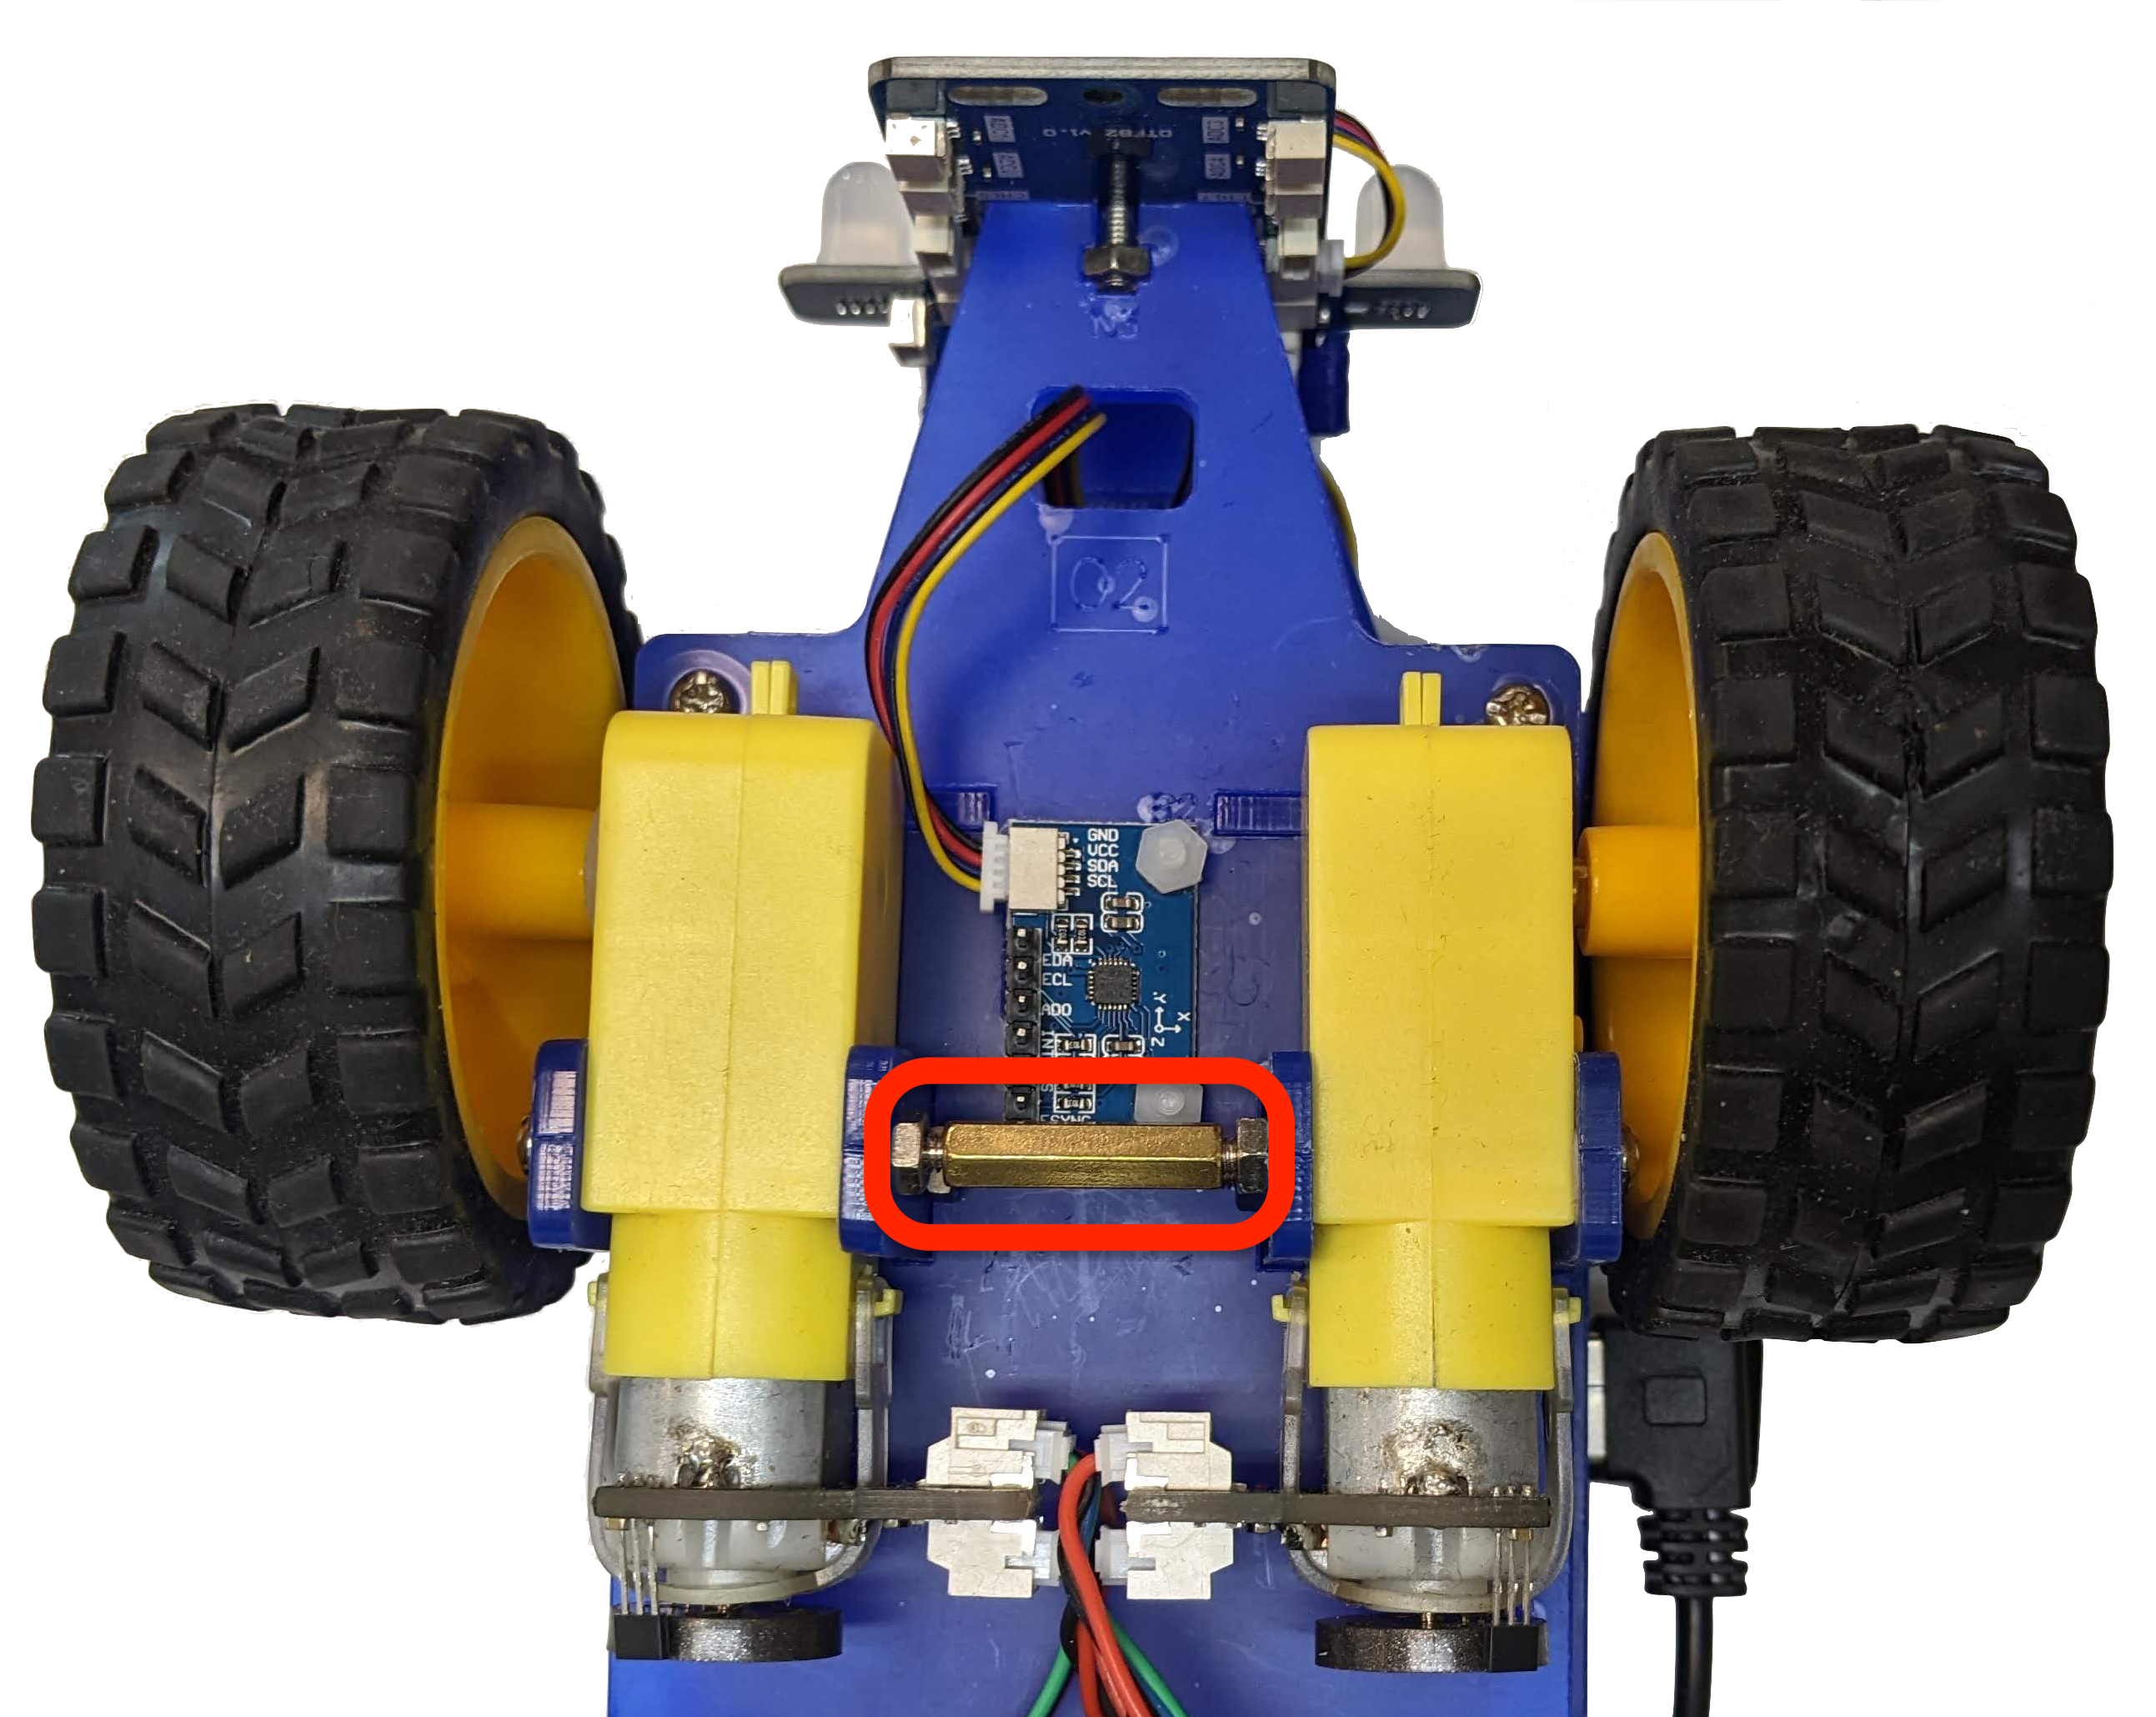
\includegraphics[width=1.0\columnwidth]{drive-upgrade.png}
    \caption{Additional crossbar to stiffen Duckiebot robot motor mounts.}
    \label{fig:stiffening-crossbar}
\end{figure}

Another way to improve the traction characteristics of the Duckiebot robots is to print an additional stiffening element\footnote{https://www.thingiverse.com/thing:2558770} that ensures the concentricity of the two motors, see Fig. \ref{fig:stiffening-element}

\begin{figure}[ht!]
    \centering
    \includegraphics[width=1.0\columnwidth]{img/duckie\_th.jpeg}
    \caption{An additional element to stiffen the motor mount of the Duckiebot robot.}
    \label{fig:stiffening-element}
\end{figure}

Reducing the negative camber of the wheels results in a significant improvement in the traction characteristics of the Duckiebot robot. It is not as sensitive to disturbances and does not change direction abruptly. Figure \ref{fig:wheel-contact} shows the effect of using an additional crossbar connecting the robot's motors. It can be seen that after using the crossbar, the Duckiebot robot wheels adhere to the surface with their entire width providing better traction.

\begin{figure}[ht!]
    \centering
    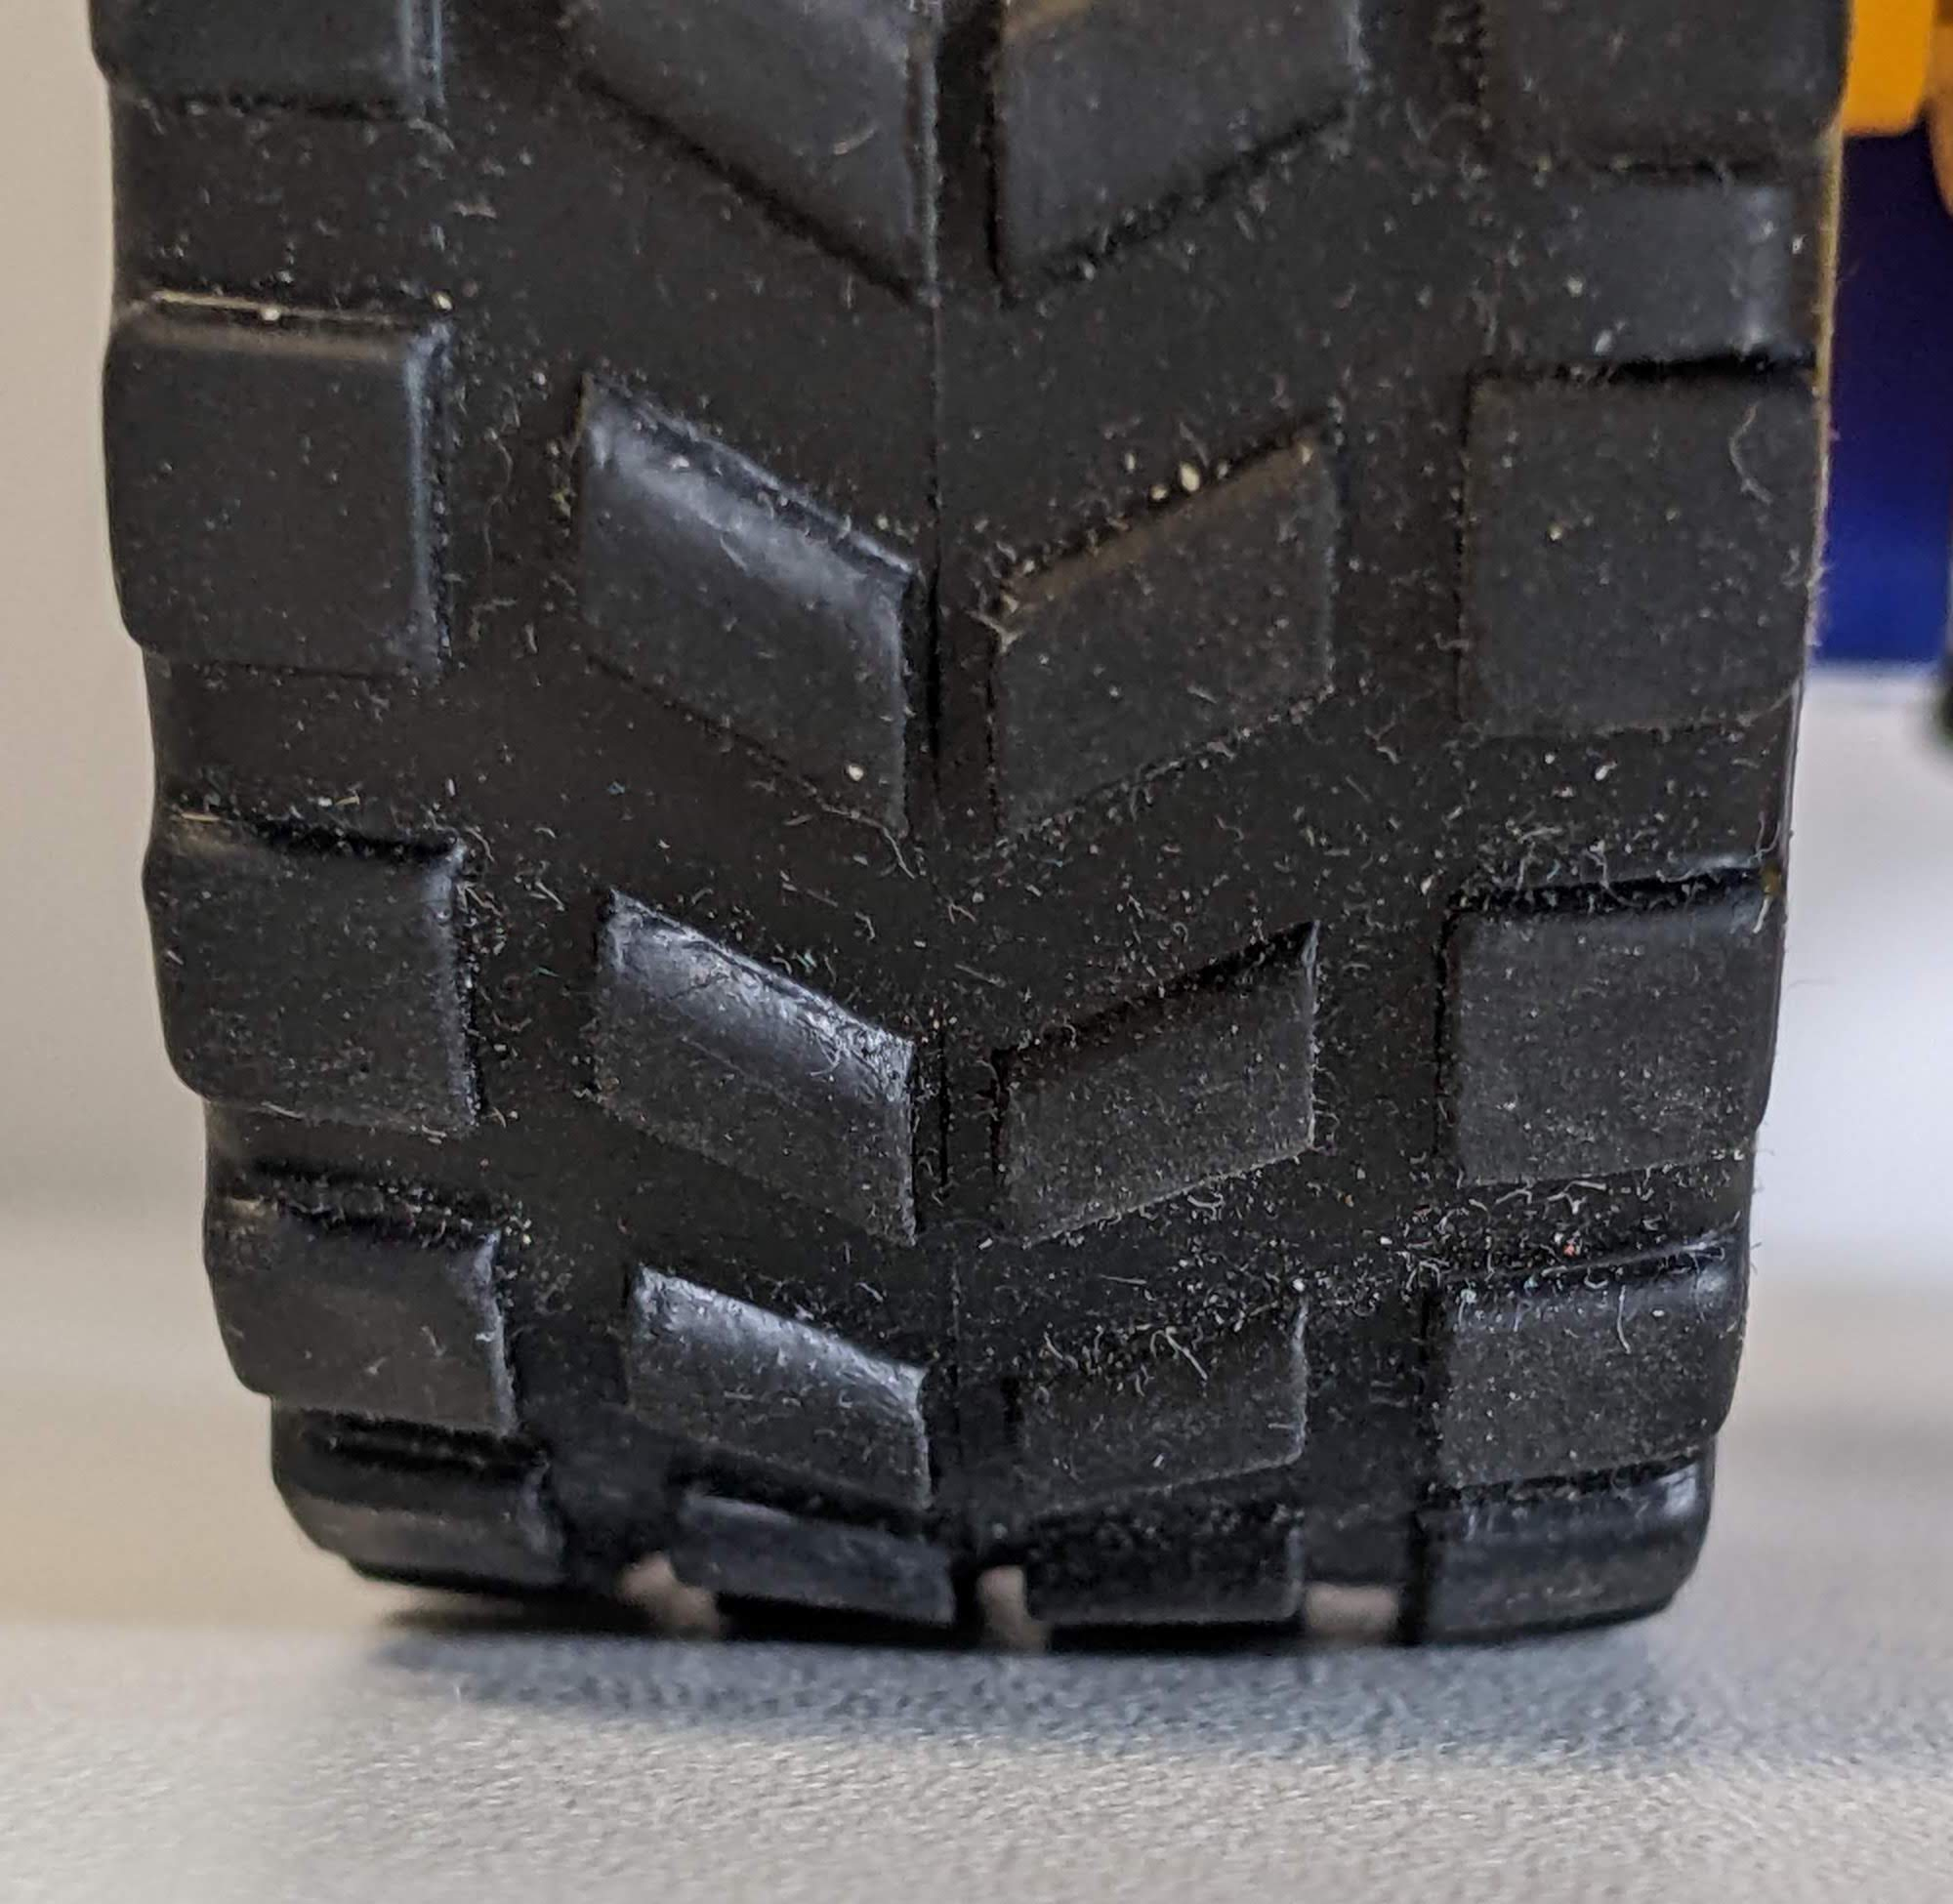
\includegraphics[width=.475\columnwidth]{wheel-contact-1.jpg}
    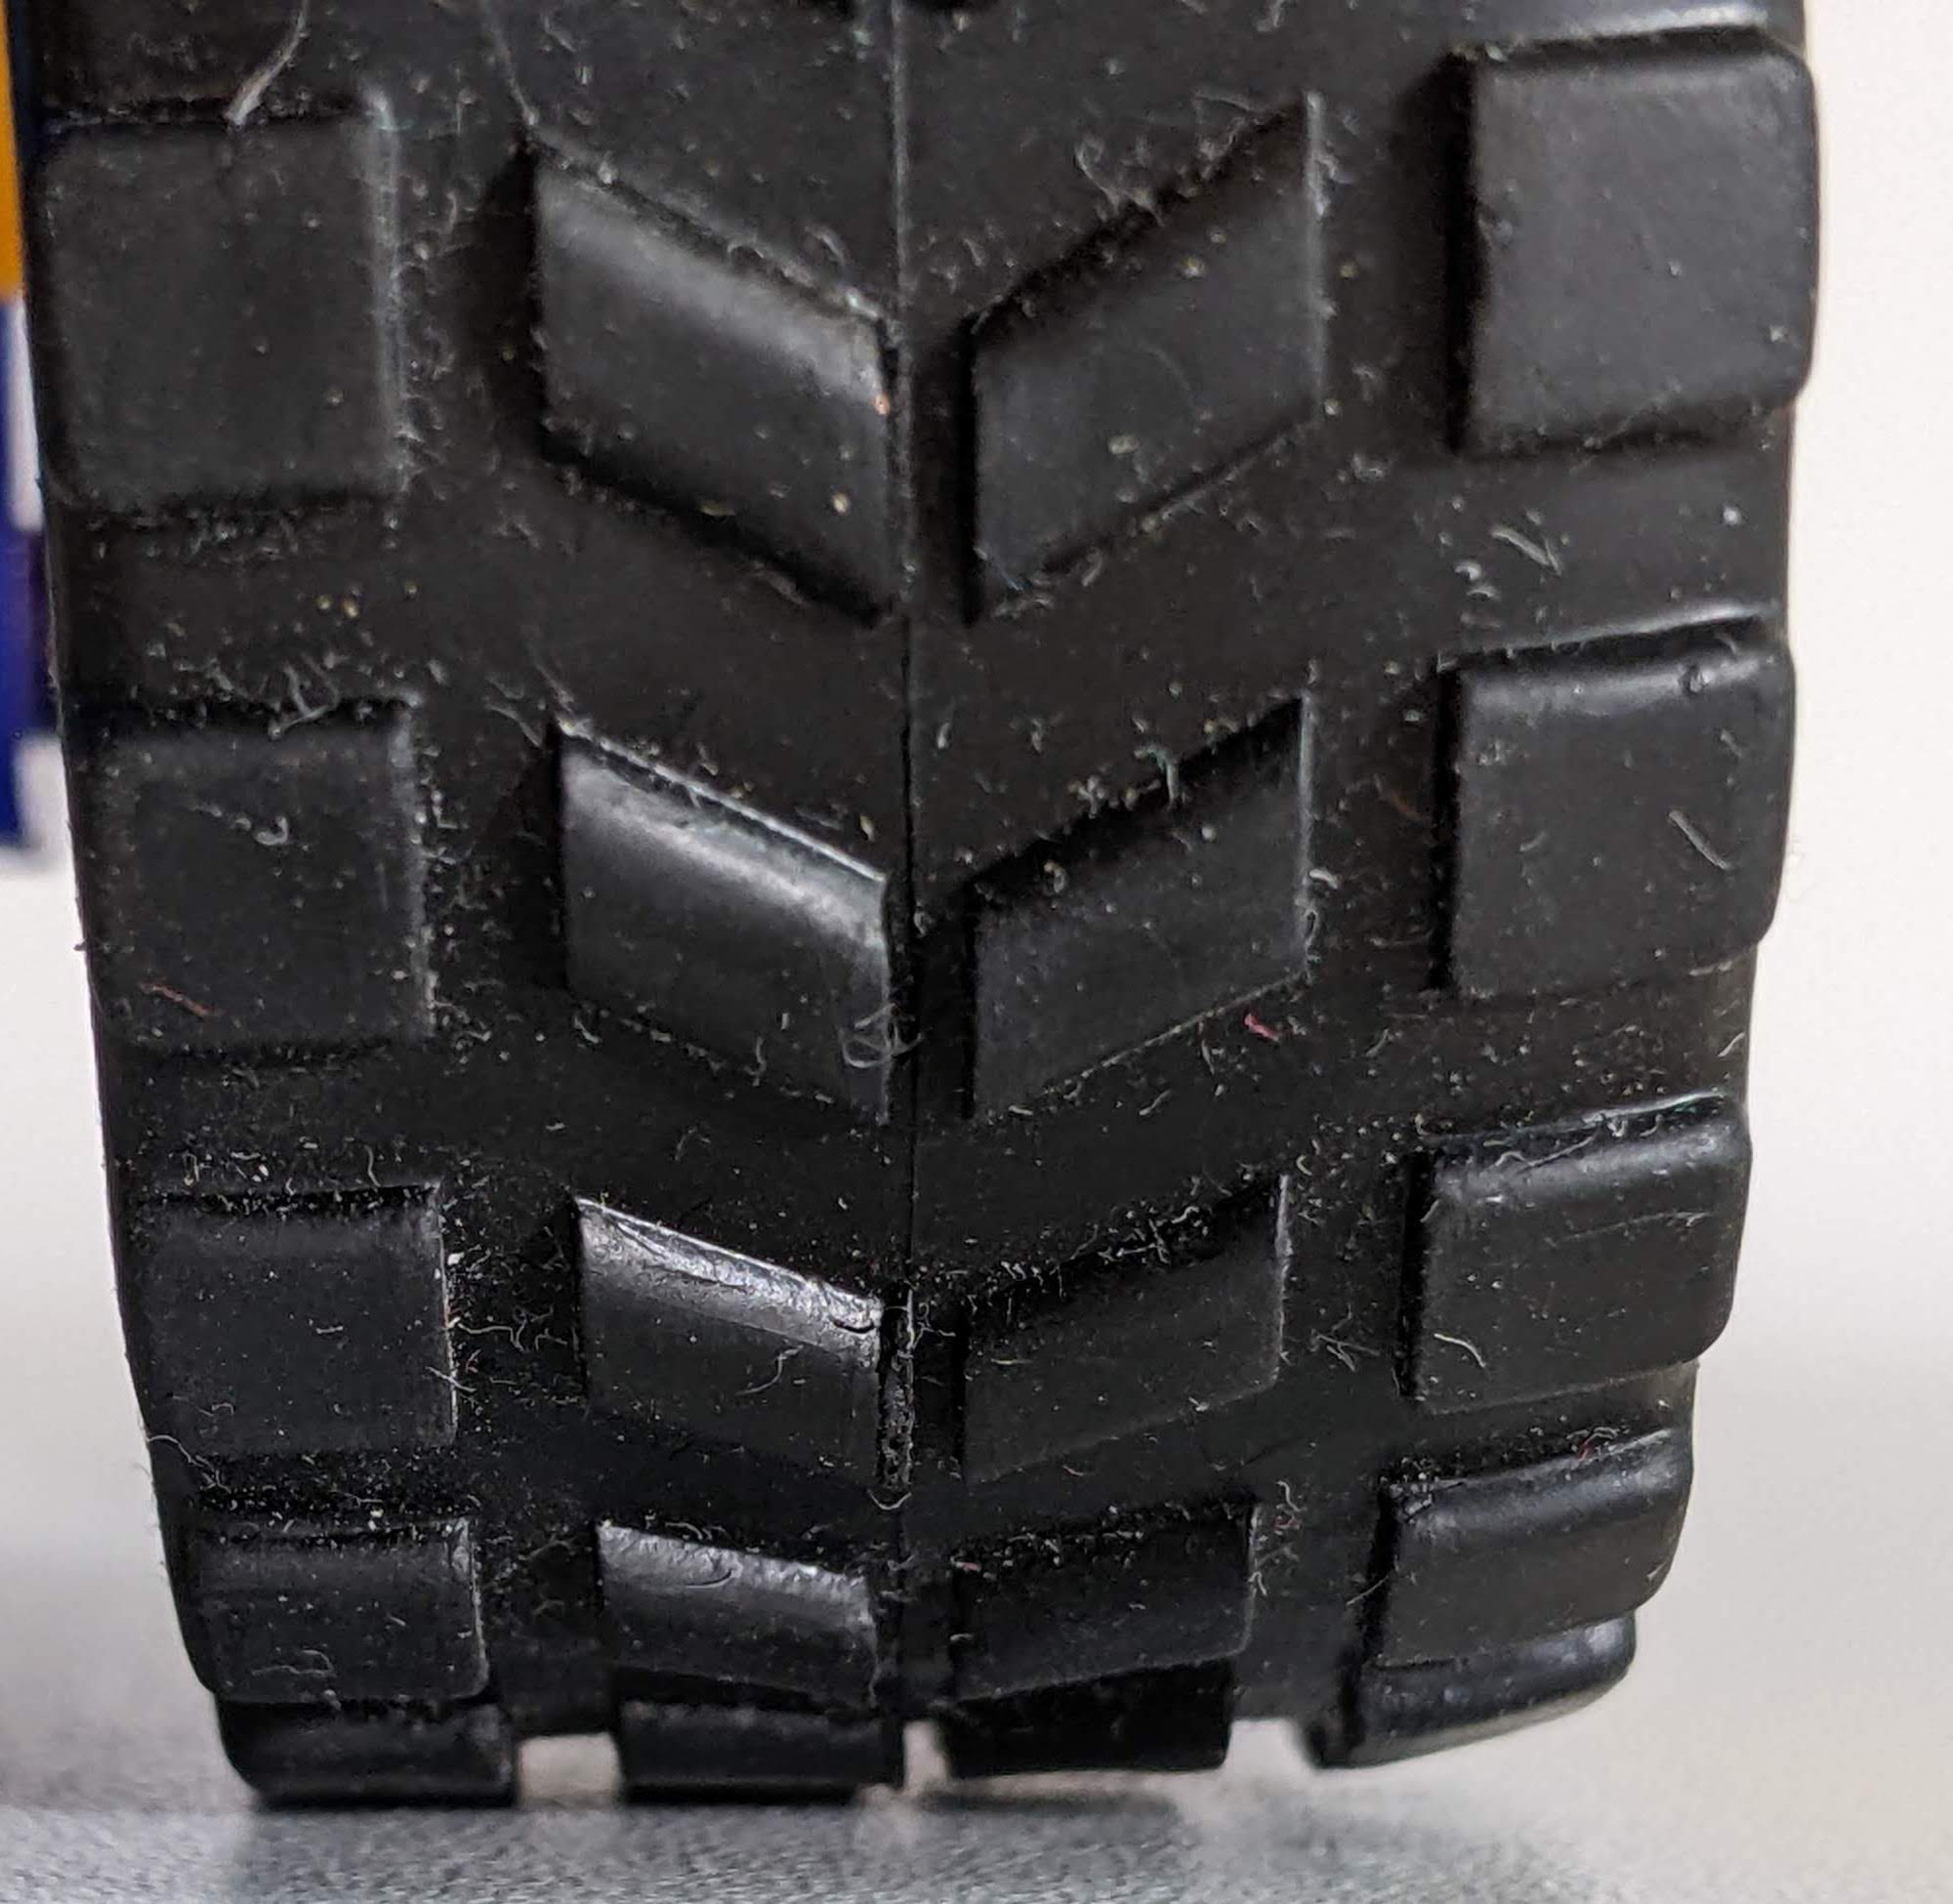
\includegraphics[width=.475\columnwidth]{wheel-contact-2.jpg}
    \caption{The result of using the crossbar to stiffen the motor mounts on the Duckiebot robot wheels.}
    \label{fig:wheel-contact}
\end{figure}

\subsection{Motors}
The original Duckiebot robots use DG01D-E motors with a gearbox of 48: 1, 90 rpm and a torque of 0.078 Nm before the gearbox and a torque of 3.744 Nm after the gearbox.
The DG01D-E is also equipped with a quadrature encoder with a probable resolution of 8 pulses per revolution (the manufacturer does not provide this information) before the gearbox and 576 pulses after the gearbox. The DG01D-E motor features high speed but not very high torque; see table \ref{table:dc-motors-summaery}. Taking into account the imperfections of the mock-up, see section \ref{subsec:plane}, and in particular the different heights between the different panels (see figure \ref{fig:smart-city-plan-1}) caused the Duckiebot robot to be able to stop while moving from one panel to another.

% https://ros-mobile-robots.com/DG01D-E-motor-with-encoder/
% https://www.cuidevices.com/blog/what-is-encoder-ppr-cpr-and-lpr
The motors in the Duckiebot robots have been replaced with SJ01 motors (SKU:FIT0450) with 120:1, 160 rpm gearing and 0.07Nm torque before gearing and 8.4 Nm torque after gearing. In addition, the SJ01 motor is equipped with a quadrature encoder with a resolution of 8 pulses per revolution before the gearbox and 960 pulses per revolution after the gearbox.  

Both motors have the same external dimensions, housings, and mounting holes, so replacing them is not a problem. You should only pay attention to the correct connection of motor control signals and encoder signals because in the DG01D-E motor all signals are integrated in one 6-pin connector, while in the SJ01 motor there are connectors: one for power supply and the other for the encoder. The \ref{table:dc-motors-summaery} lists all the parameters of the DG01D-E and SJ01 motors.  

\def\arraystretch{1.5}
\setlength{\tabcolsep}{0.0175\columnwidth}
\begin{table}[ht!]
\begin{center}
    \begin{tabular}{|c|c|c|c|c|c|c|c|}
    \hline
         \multirow{3}{*}{\thead{Motor\\type}} & \multirow{3}{*}{n} & \multicolumn{3}{|c|}{before gearbox} & \multicolumn{3}{|c|}{after gearbox} \\ \cline{3-8}
         
         & & $\omega$ & torque & encoder & $\omega$ & torque & encoder  \\
         
         & & [rpm] & [Nm] & [ppr] & [rpm] & [Nm] & [ppr]  \\
         \hline \hline
         DG01D-E & 48:1 & 90  & 0.078  & 12   & 1.874 & 3.744 & 576  \\ 
         \hline
         SJ01 & 90:1 & 120  & 0.070  & 8 & 1.333  & 8.400  & 960 \\ 
         \hline
    \end{tabular}
    \caption{\label{table:dc-motors-summaery}Parameters of Duckiebot robot motors.}
\end{center}
\end{table}

Finally, the SJ01 motor, despite having slightly less torque in front of the gearbox, is definitely a better choice than the DG01D-E motor. Final has more torque and a higher resolution encoder, which definitely improves the driving characteristics of the Duckiebot robot and the accuracy of motor speed control. The slightly lower speed of the $\omega$ after gearing does not matter at all, because Duckiebot robots are not robots that are supposed to participate in robot races, but are supposed to intelligently move around the city mock-up.

%\todo{Sprawdzić czy SJ01 ma metalowy wał, jeśli tak dodać zanie, że można dodatkowo przykręcić koła do }

%\href{https://botland.com.pl/silniki-dc-z-przekladnia-i-enkoderami/6287-silnik-z-przekladnia-sj01-120-1-6v-160rpm-enkoder-5904422306793.html}{Botland}, \href{https://www.dfrobot.com/product-1457.html}{DFRobot}

\subsection{Battery}
The Duckiebot robots use a lithium ion battery with a capacity of 10Ah. The battery case also contains a built-in electronic circuit that controls the battery's operation, e.g. does not allow it to over-discharge, which is known to be harmful for this type of battery. The battery control itself is much more complex, as can be seen by analyzing the state machine implemented by the battery electronics; see Fig. \ref{fig:battery-state-machine}.

\begin{figure}[ht!]
    \centering
    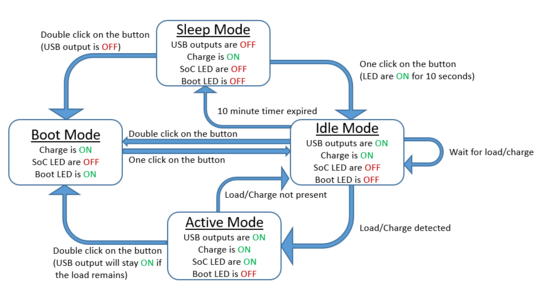
\includegraphics[width=1.0\columnwidth]{BatteryStateMachine.png}
    \caption{State machine implemented in Duckiebot robot's battery control electronics.}
    \label{fig:battery-state-machine}
\end{figure}

The state of charge of the battery, as well as the current state of the state machine in which the battery is located, is presented by means of 4 leds mounted on the case. This is a simple but effective solution. Unfortunately, in the Duckiebot robot itself, the battery is built in such a way that the LEDs indicating the battery status are not visible, which makes it impossible in any way to determine, for example, how low the battery of the Duckiebot robot is. It is also possible to read the battery level of the Duckiebot robot by software, unfortunately, very often this functionality does not work properly. The simplest solution to this problem is to change the way the battery is built into the Duckiebot robot so that its status can always be read using the LEDs mounted on the housing. 

\subsection{Mock-up}\label{subsec:plane}
One of the main elements of the Duckietown project is a mock-up. It is intended to model the shape of the road, the layout of intersections on which Duckiebot robots move. Straight lines and curves are marked with white and yellow lines, whereas intersections are marked with red lines. The route along which the Duckiebot robots move can be freely configured by an appropriate arrangement of elements of the mock-up. The basic element from which the route is built is a rubber-foam mat. The first problem is the peeling off parts of the tape used to mark the lines, see Fig. \ref{fig:smart-city-plan-1}. The second problem is the sheer quality of the rubber foam panels. The panels from one package have different heights, which results in the Duckiebot robots moving on them changing their direction of travel in a completely random manner; see Fig. \ref{fig:smart-city-plan-1}.

\begin{figure}[ht!]
    \centering
    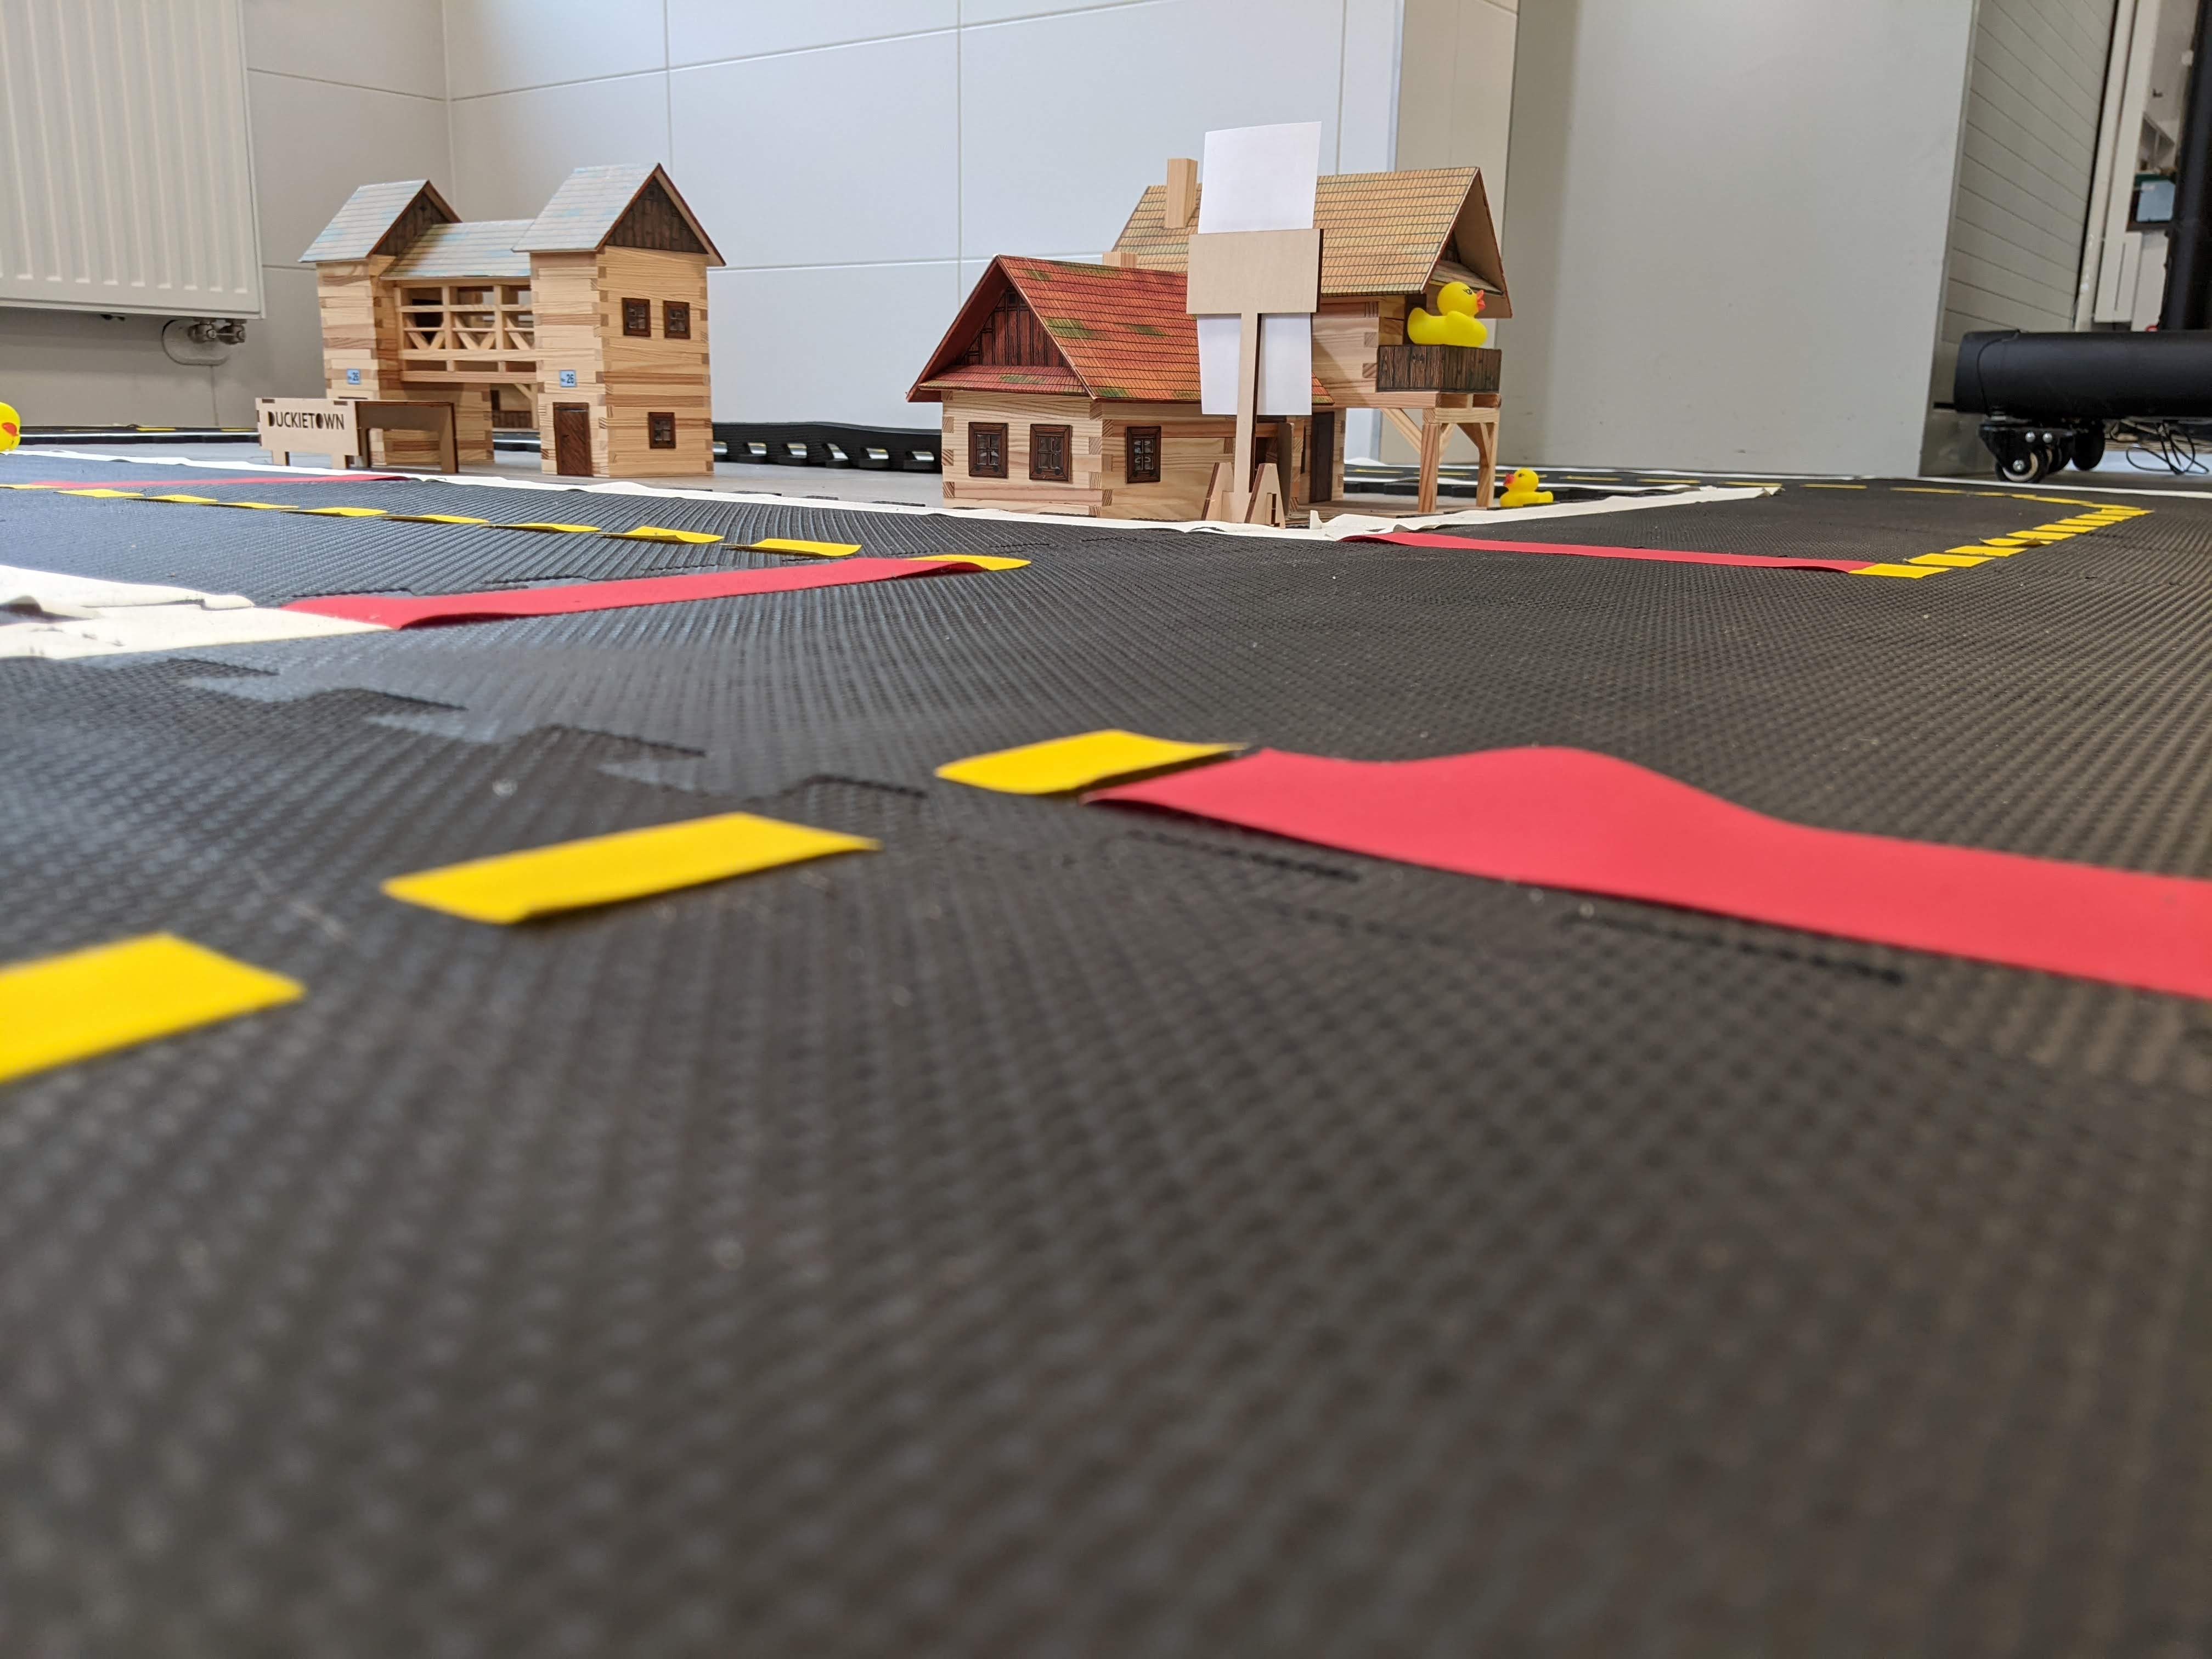
\includegraphics[width=.475\columnwidth]{floor-1.jpg}
    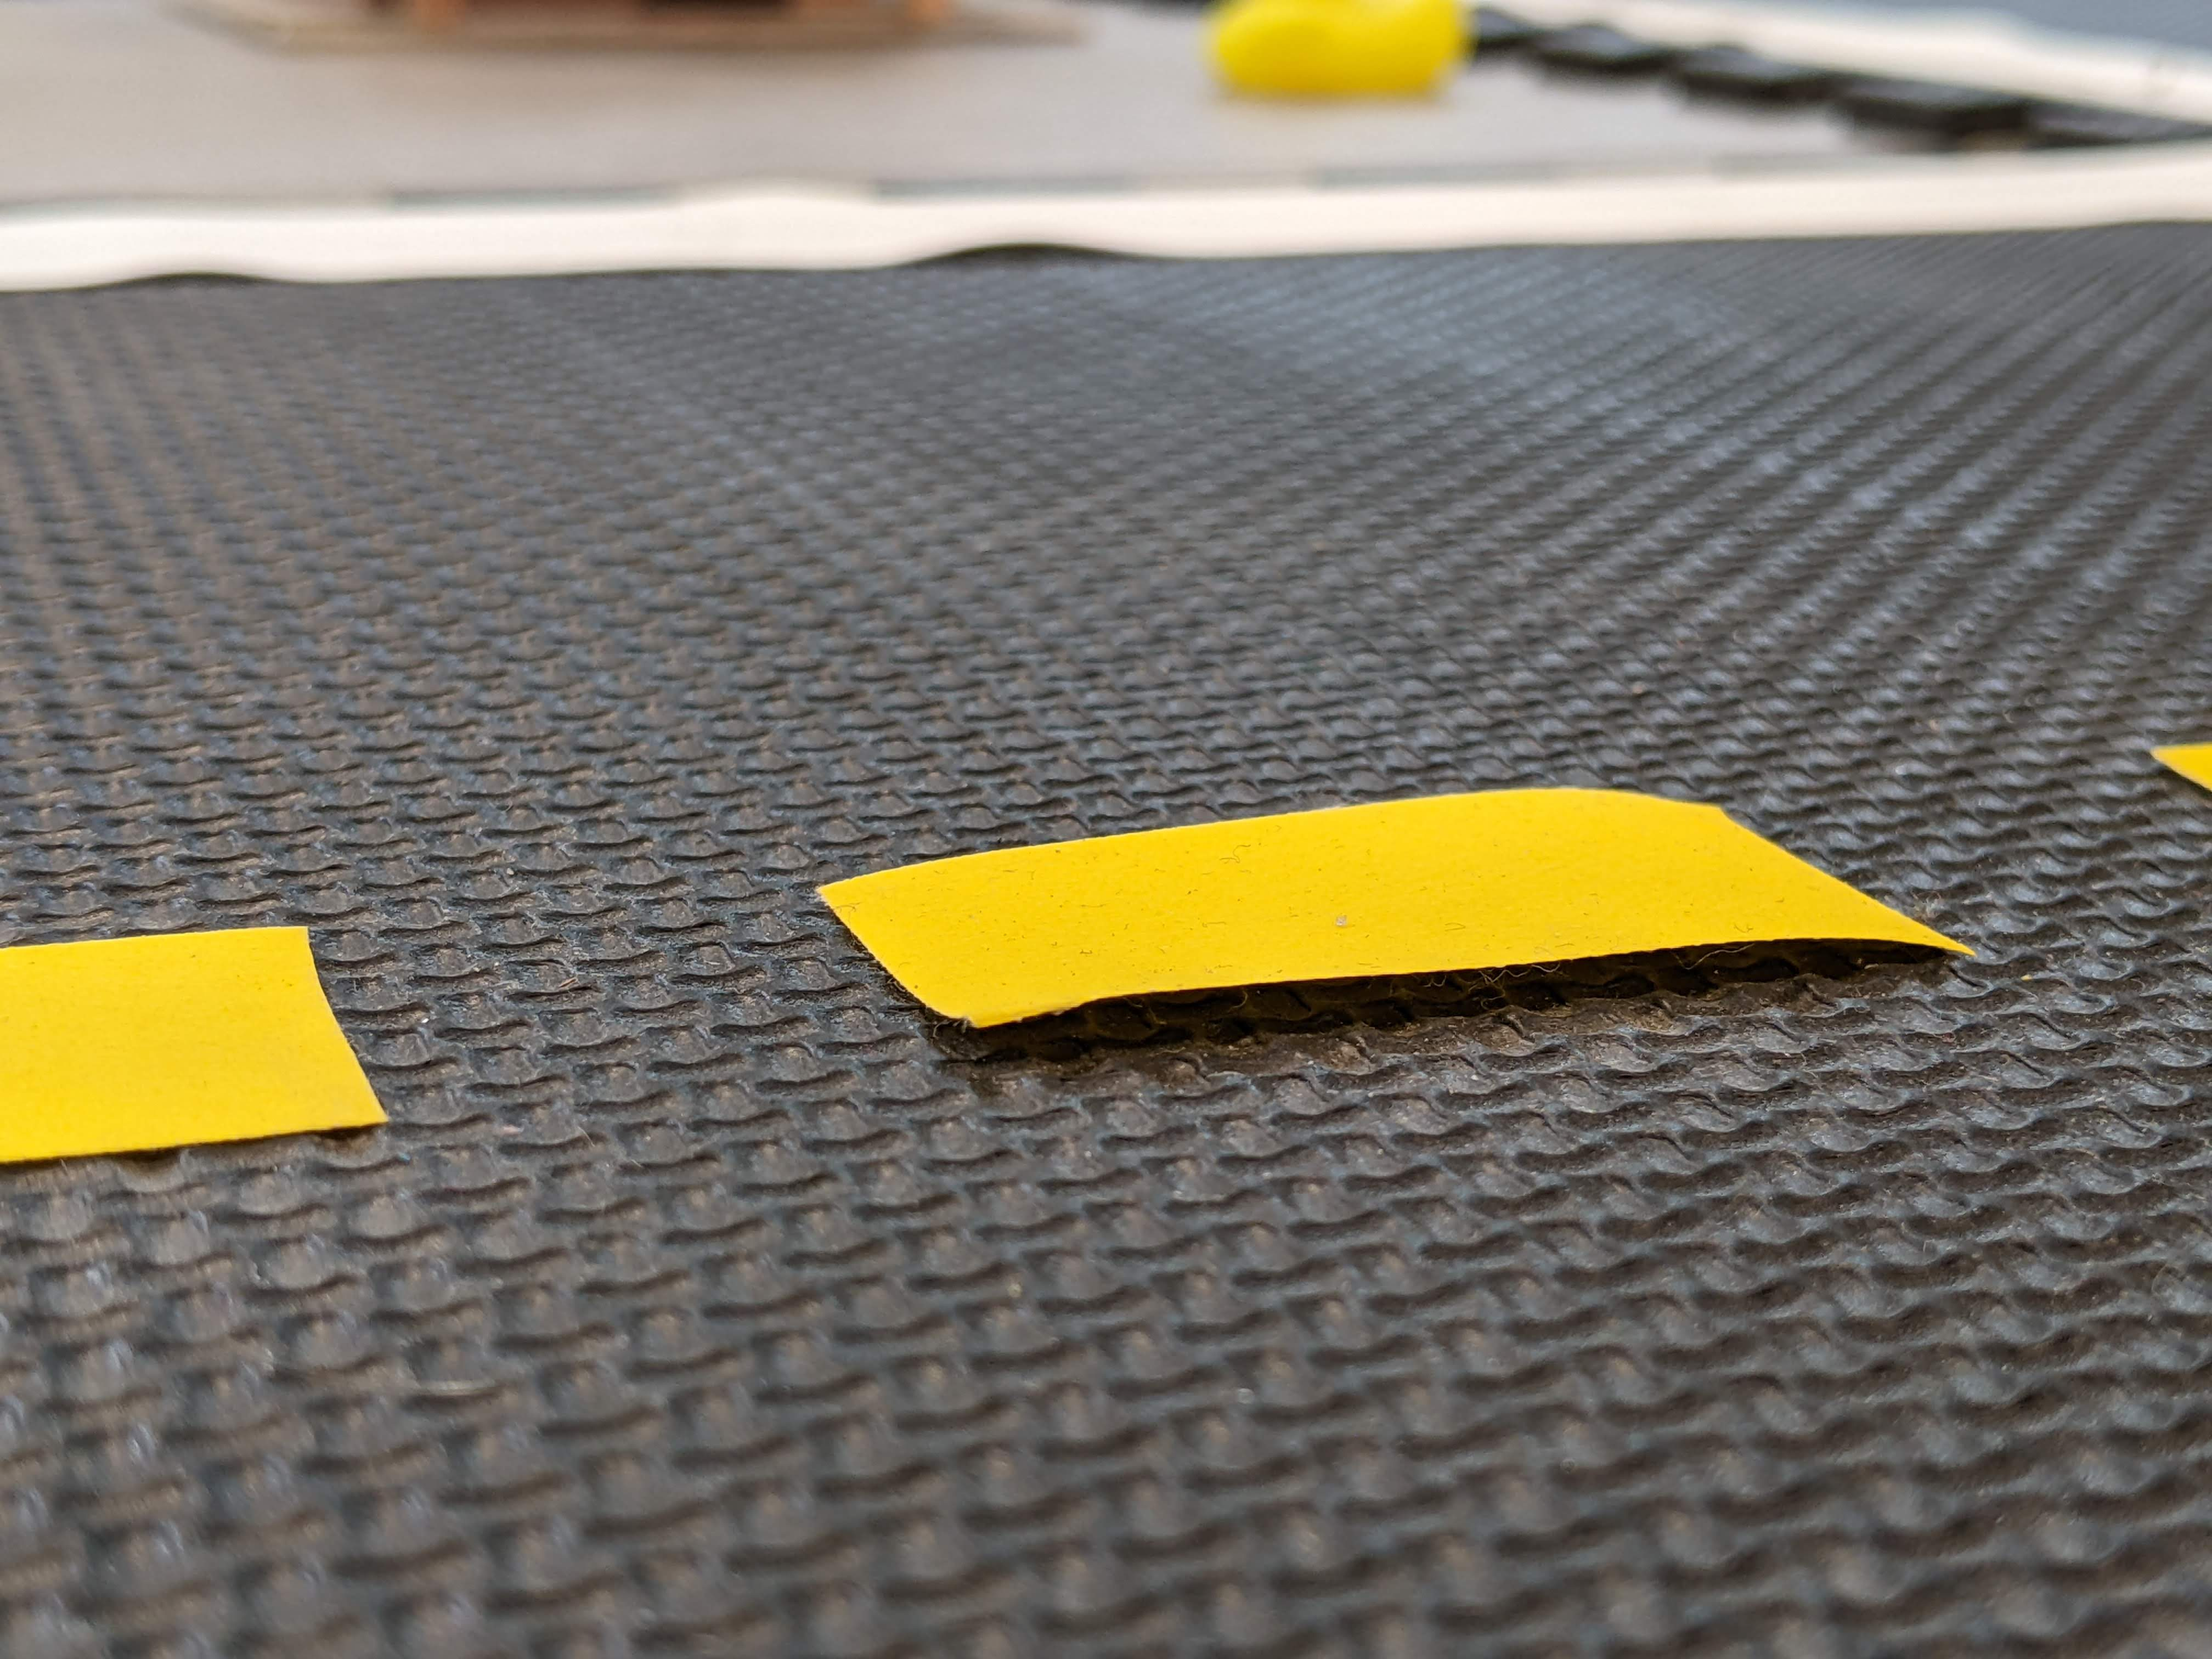
\includegraphics[width=.475\columnwidth]{floor-2.jpg}
    \\
    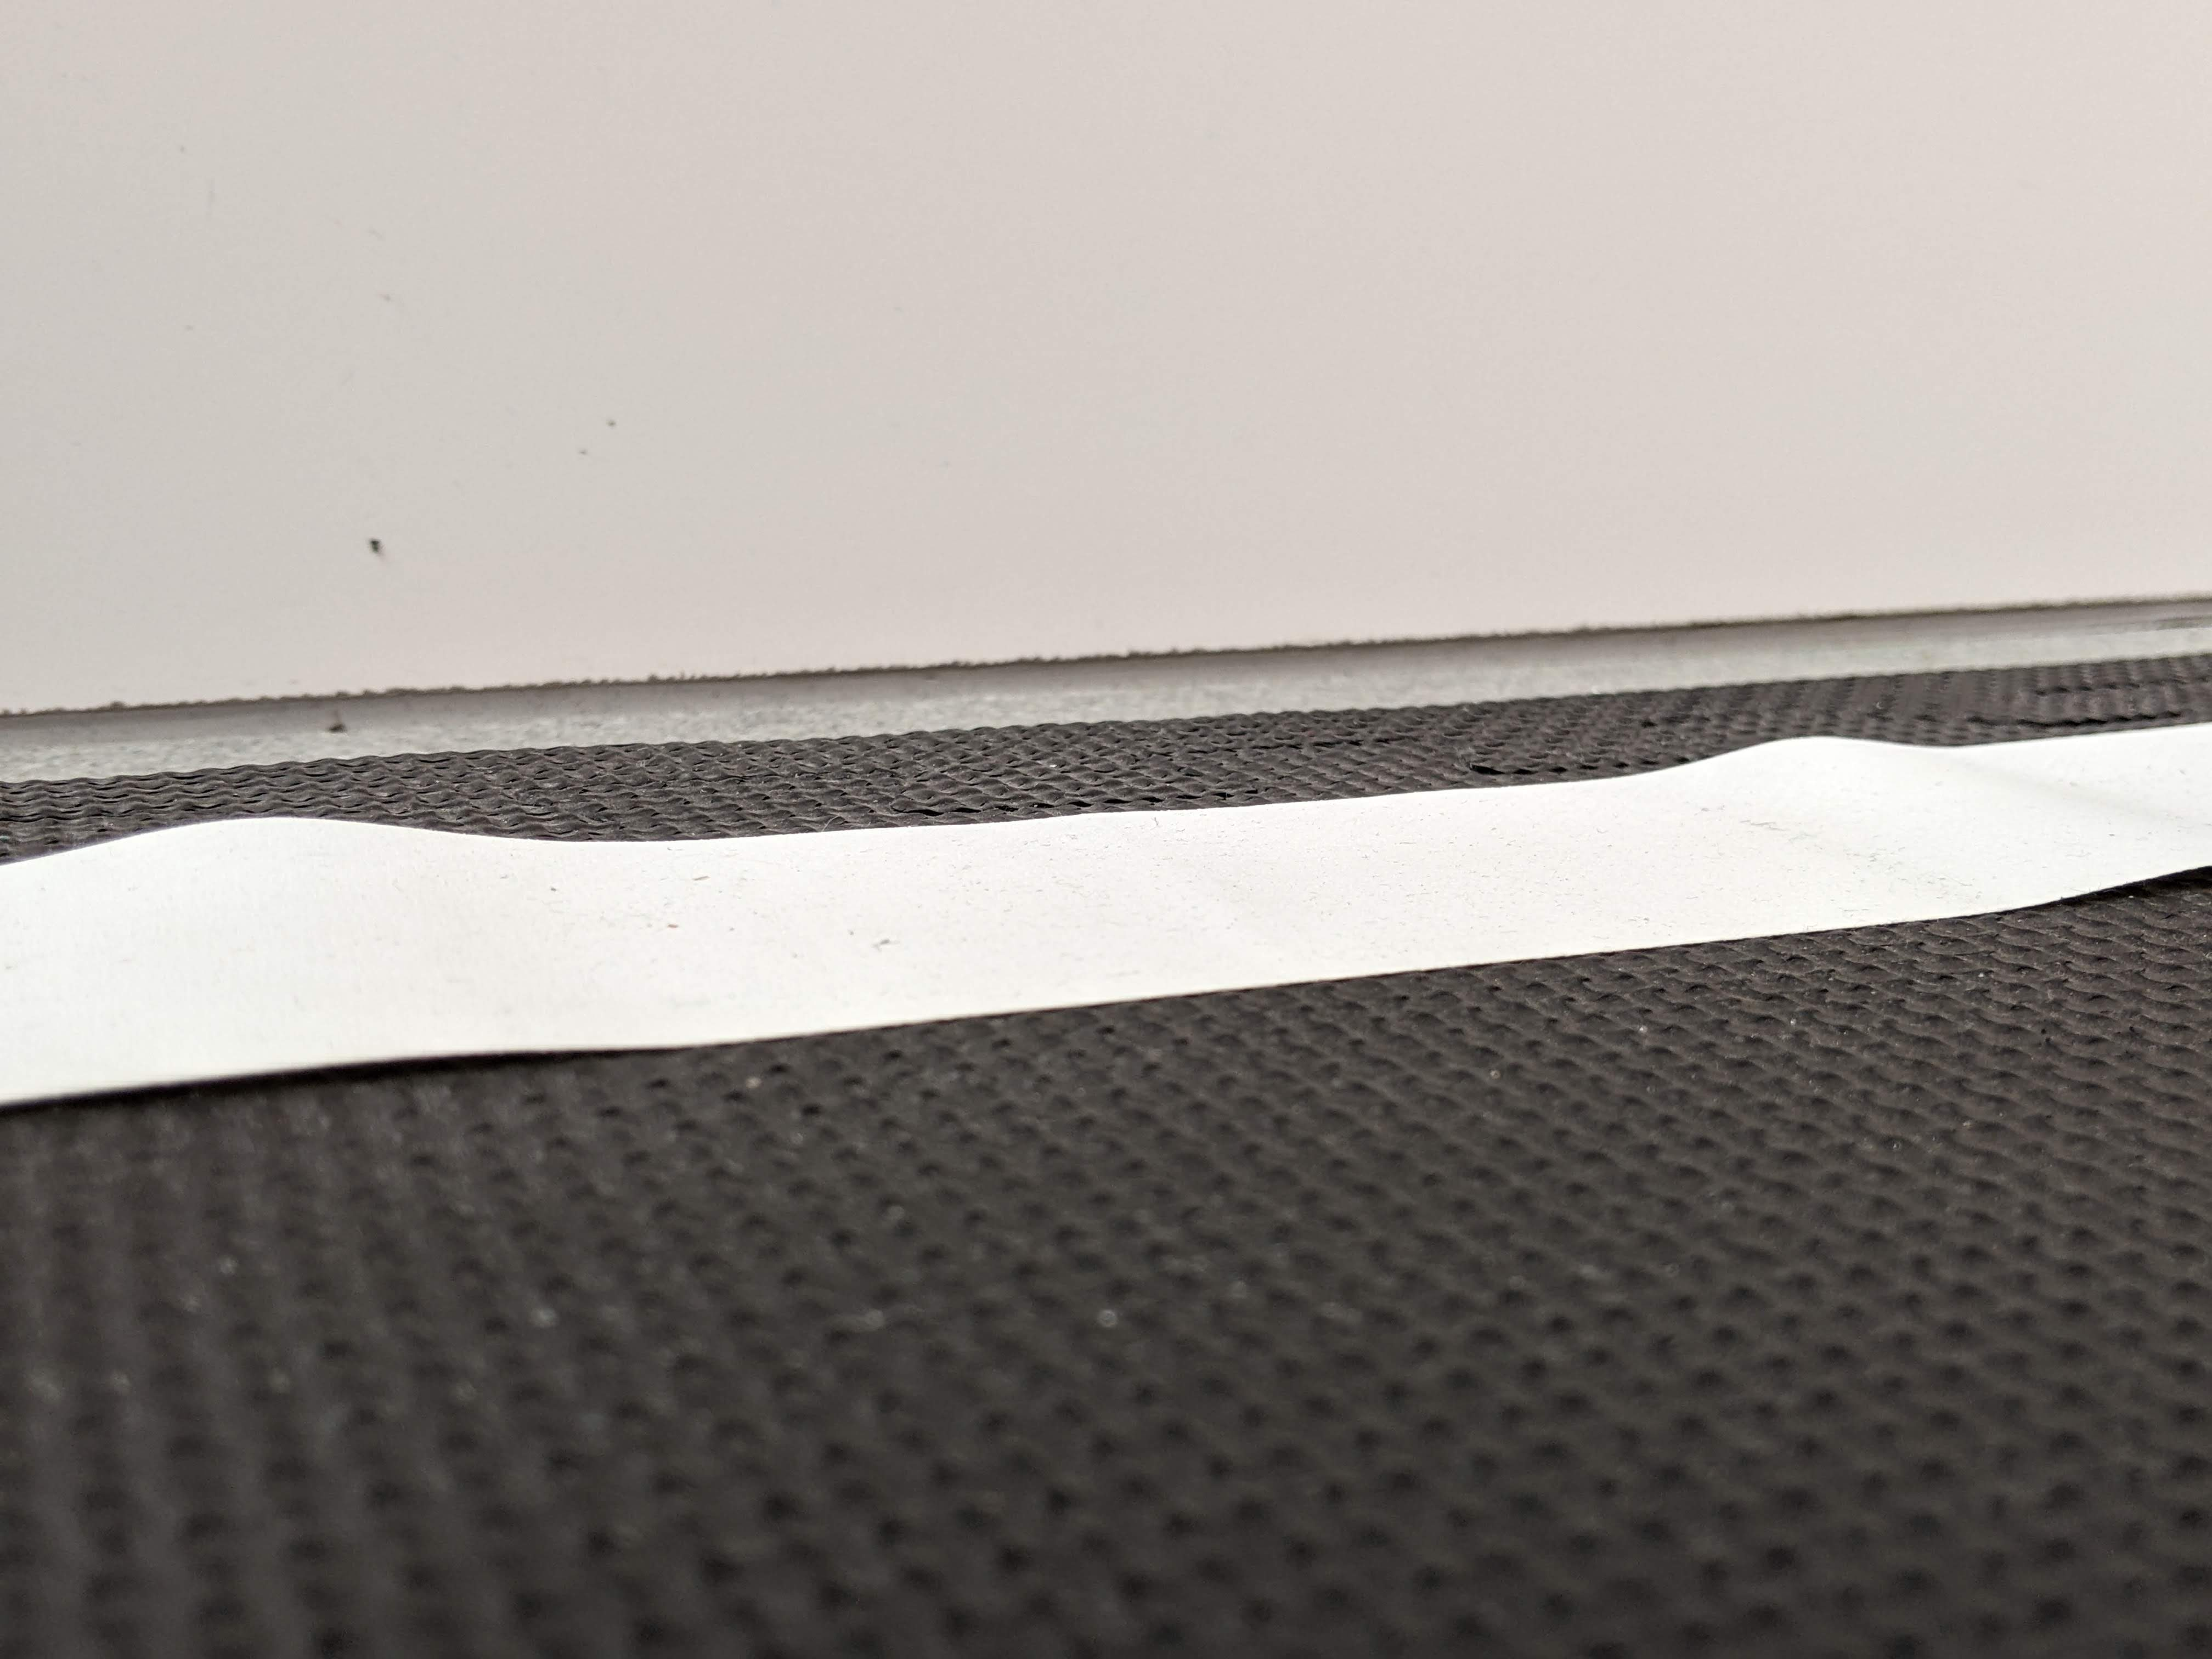
\includegraphics[width=.475\columnwidth]{floor-3.jpg}
    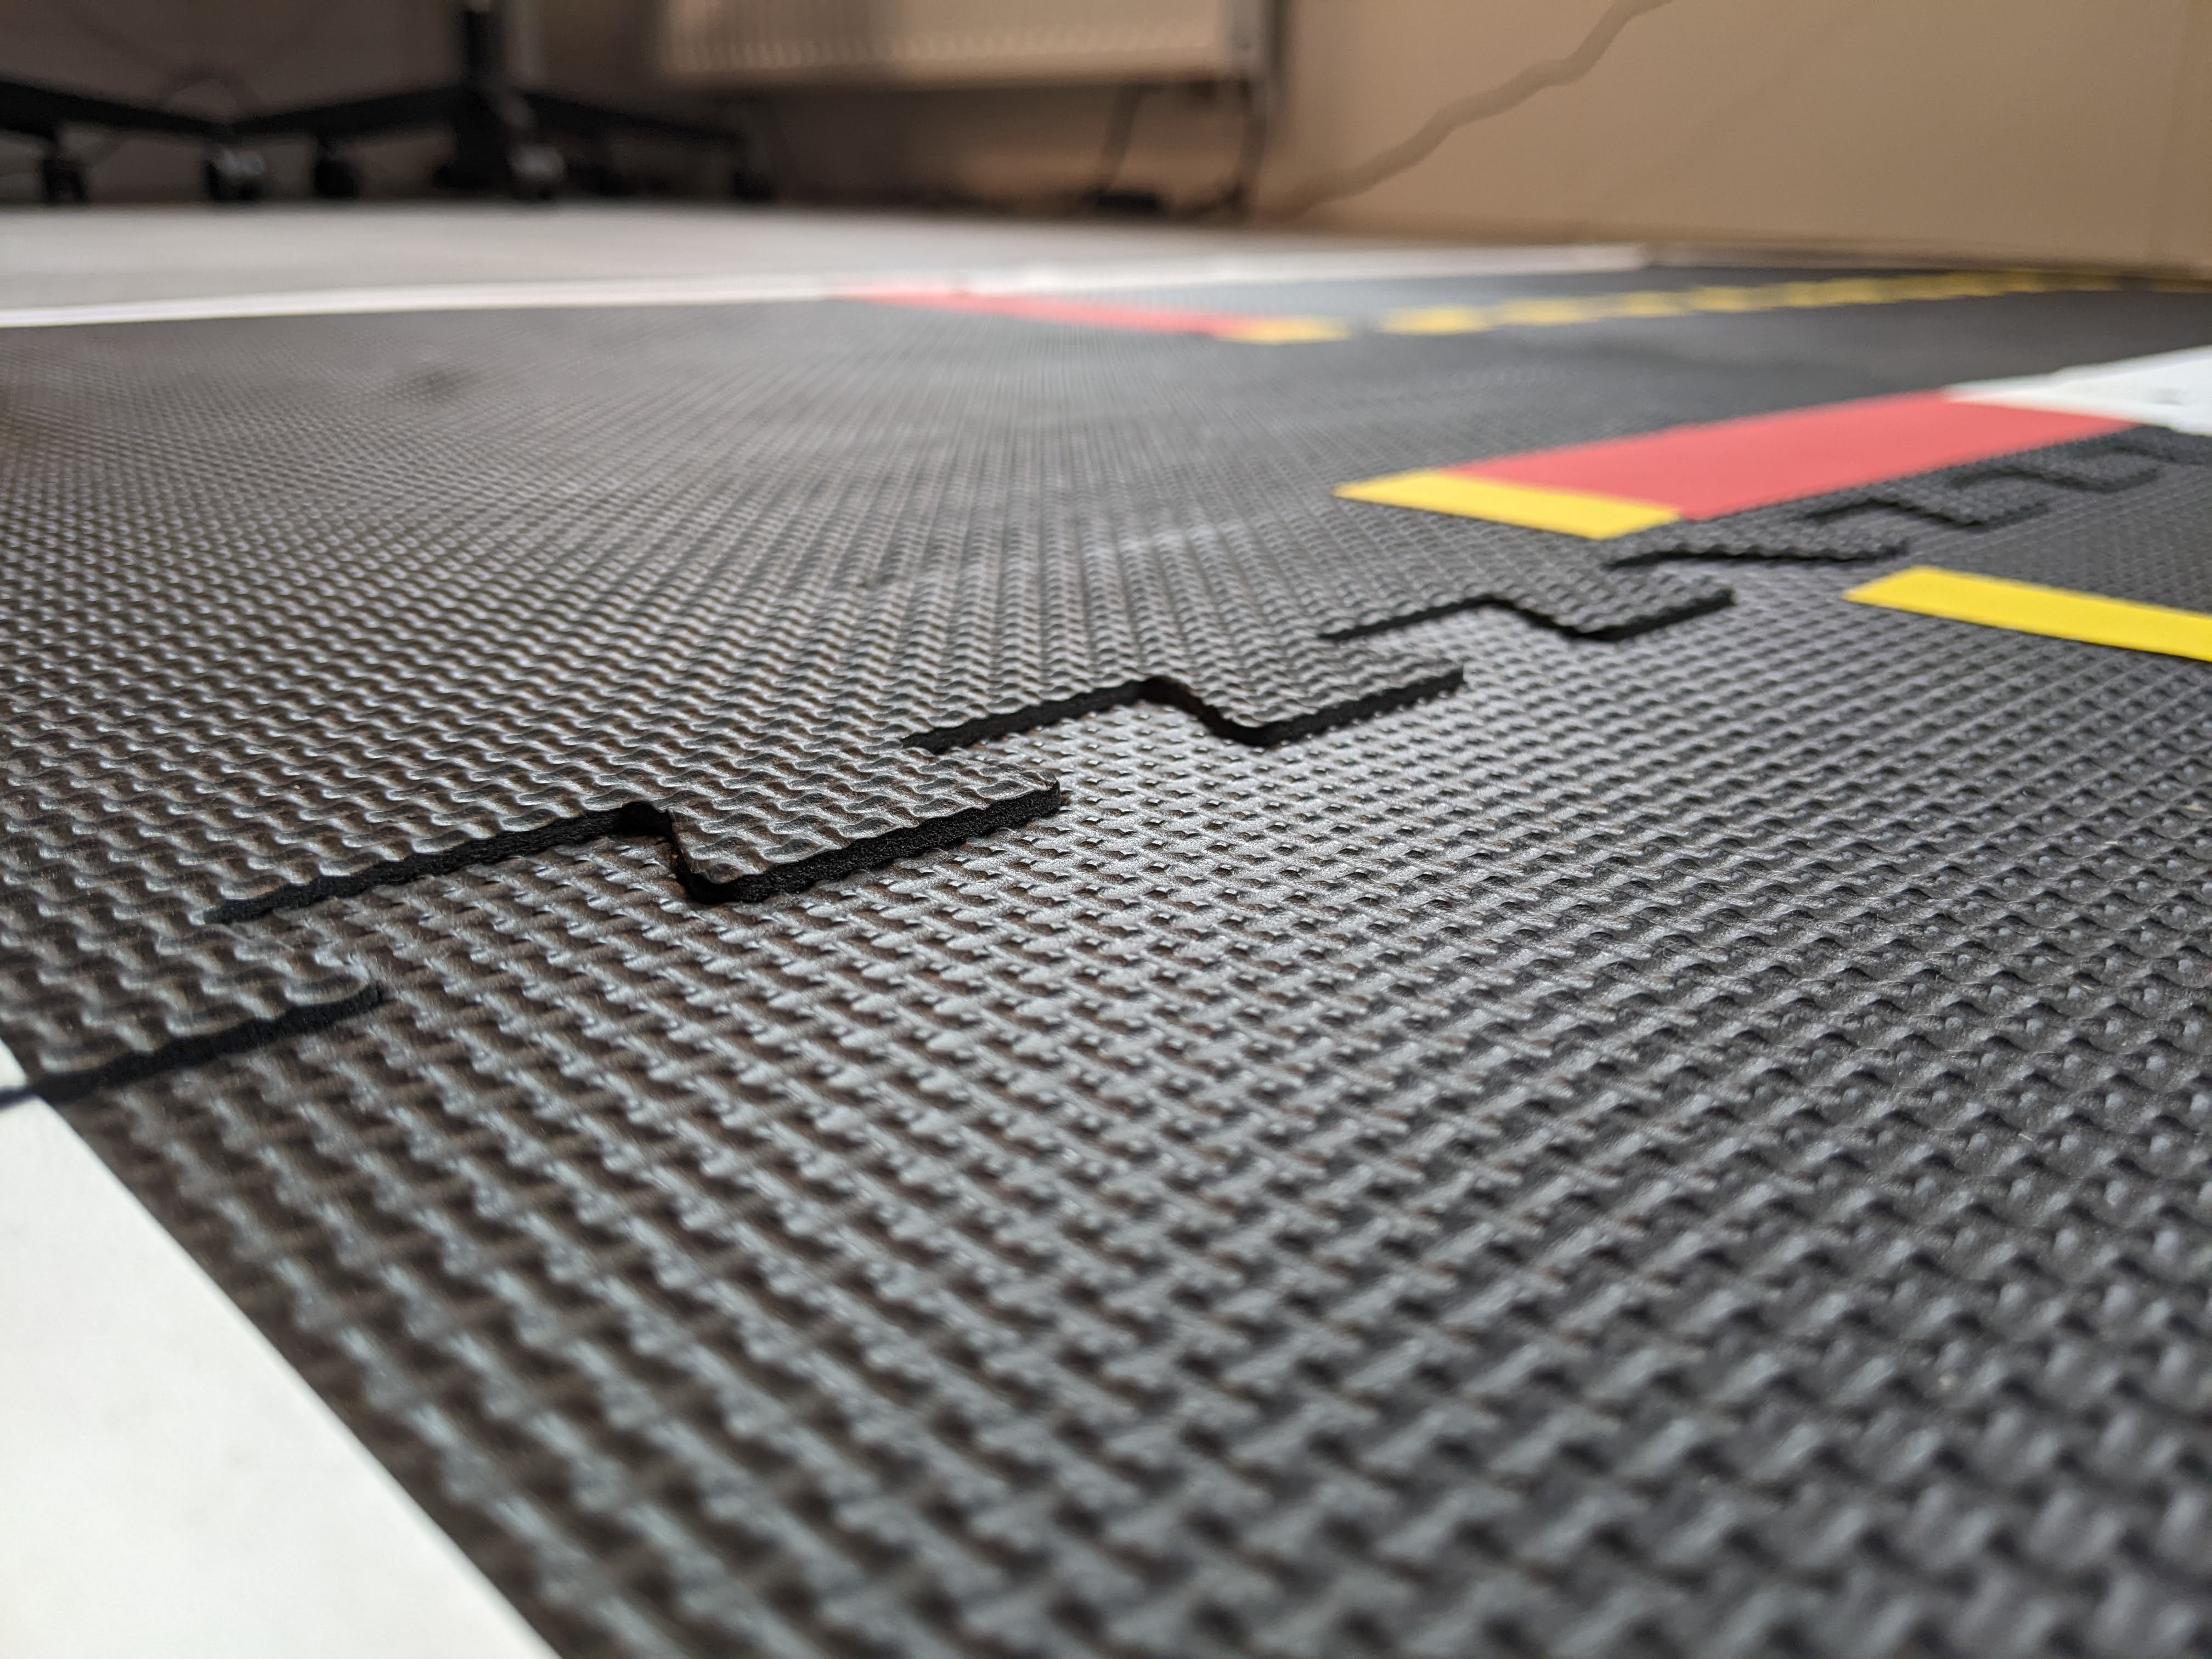
\includegraphics[width=.475\columnwidth]{floor-4.jpg}
    \caption{Details of the Duckietown project mock-up.}
    \label{fig:smart-city-plan-1}
\end{figure}

The solution to the mat problems is first of all to use a different tape than the one sold by the Duckietown Foundation. Among the various tapes tested by the authors, the best properties were characterized by the tape of WELSTIK company. In addition, before the tape is adhered to the panel, it is worth cleaning it, for example, with isopropyl alcohol or other liquid that in its composition contains alcohol to degrease the surface. The last operation that can be performed is to heat the glued tape using, for example, a hair dryer. 

\section{Software}\label{sec:software}
Definitely the strong point of the Duckietown project is its software, for which the most popular framework for robot programming at the moment was used: Robot Operation System. 
The division of the entire software into individual modules and packages is correct, understandable, and logical. 
The individual elements/modules of the software are realized using containerization technology. Thanks to the widespread use of containerization, you can easily, quickly, and safely create and test your own software. It is also worth noting that software development technologies that use containerization are now very popular and are often used in software development.  

The Duckietown project software also includes the DuckieTown Shell. This is a set of scripts that facilitates and automates various activities related to the day-to-day operation of Duckiebot robots, e.g.: updating software, creating docker images, running containers, and much more.

The state in which the Duckiebot robot is currently in can be checked using software in a web browser. Each Duckiebot robot provides such an interface in the form of a microservice.

Duckiebot robots can be programmed in Python or C/C++, which is a consequence of using the ROS framework. The source code for the Duckiebot robot software is available as a repository on github\footnote{https://github.com/duckietown}.

In fact, the only drawback of the currently available programming is the inability to use the GPU that the NVIDIA Jetson Nano computer is equipped with. This is primarily due to the incompatibility of the python software version, tensorflow. The possibility of using a hardware GPU affects primarily the use of neural networks to control the Duckiebot robot.

\section{Documentation}\label{sec:documentation}
Documentation of the Duckietown project consists of electronic documents (in html or pdf format) in which issues ranging from the assembly of the Duckiebot robot (step by step), the correct execution of the mock-up, to issues related to robot programming are described in an easy and accessible manner.
In the documentation you can find comprehensive descriptions of the software architecture of the Duckietown project, a great number of examples and also recommendations for dealing with problems. Duckietown project documentation is also updated on an ongoing basis, e.g. inactive links are corrected (after they were reported), and additional information is added.
Unfortunately, the documentation of the Duckiebot project is not yet complete; many of its sites are missing content that is not being completed for the time being.
The Duckiebot project documentation also includes teaching materials in the form of lectures, videos, exercises, as well as a comprehensive course on the \emph{edX} e-learning platform titled \emph{"Self-Driving Cars with Duckietown."} Exercises in the form of jupyter scripts and github repository templates are also prepared for use in class.

\section{Conclusion}\label{sec:conclusion}
In conclusion, it should be said that the Duckietown project, despite its many flaws, is a worthwhile project. Undoubtedly, the greatest advantage of the Duckietown project is that it represents a complete ecosystem that includes: documentation, software, hardware and a simulation environment that enables effective and modern teaching and advanced scientific research in the field of autonomous robots. 

The numerous flaws perceived and described in the article can be easily corrected on their own. It should also be noted that the managers of the Duckietown project, after reporting problems to them and suggesting solutions, keep updating the project documentation with proposed solutions. 

In the opinion of the authors, the most urgent things that should be improved are: the mechanical design of the body (better materials, a different way of connecting and fixing various components), replacing the engines with a different model, and updating the software so that it is possible to use the GPU hardware. With time, it will also become necessary to replace ROS with its newer version ROS2.


\bibliographystyle{IEEEtran}
\bibliography{references}

\end{document}
